\documentclass{beamer}
\usepackage{caption}
\usepackage{subcaption}
\usepackage{slashed}
\usetheme{Luebeck}
\setbeamertemplate{navigation symbols}{}
\setlength{\parskip}{2.5mm}
\title[Dilepton $t \bar{t}$ estimation\hspace{14em}\insertframenumber/18]{Di-lepton $t \bar{t}$ estimation from \\ Semi-leptonic $t \bar{t}$ in SUSY searches}
%\author{\emph{Tim Brooks}, Glen Cowan, Aftab Alam}
\author{\emph{Tim Brooks}, Glen Cowan}
\institute{Royal Holloway University of London}
\date{28/8/12}
\begin{document}

\begin{frame}
\titlepage
\end{frame}

\section{Search}
\begin{frame}{Dilepton SUSY search}
Search for Supersymmetry in the $2 \text{lepton} + E_{T}^{\text{miss}} + \text{jets}$ channel:
  \begin{itemize}
    \item SUSY signals can give multi-object final states
    \item $E_{T}^{miss}$ is a powerful discriminator for R-parity preserving models
    \item Di-lepton signatures can identify weak gaugino and/or slepton production
  \end{itemize}
\end{frame}

\begin{frame}{Dilepton SUSY search}
  \begin{figure}
    \centering
    %\def\svgwidth{\columnwidth}
    \includegraphics[scale=5.0]{img/susy.pdf}
  \end{figure}
\end{frame}

\begin{frame}{Dilepton SUSY search}
Additional jets in events also give power for hierarchies with large mass gaps.

Length of hierarchy determines the number of detectable jets. Most searches looks for 2 or 3 hard jets in addition to the leptons + $E_{T}^{miss}$.

The largest background to these searches is usually $t\bar{t}$.
\end{frame}

%\begin{frame}{Backgrounds}
%Several standard model processes produce similar multi-object states:
%
%\begin{table}
%\centering
%\begin{tabular}{l||c|c}
%                     & Real leptons               & Fake leptons         \\
%\hline \hline
%Real $\slashed{E}_{T}$ & $t\bar{t}$, Diboson + jets & W + jets, Single top \\
%\hline
%Fake $\slashed{E}_{T}$ & Z + jets                   & W + jets, QCD        \\
%\end{tabular}
%%\caption{This table shows some data}
%\label{tab:myfirsttable}
%\end{table}
%
%$t\bar{t}$ is normally the largest background.
%\end{frame}

\section{Control sample}

\begin{frame}{Backgrounds}
Need to measure dilepton $t\bar{t}$ in search region. Current approaches tag dilepton $t\bar{t}$ using known properties of decay.

Our approach - measure semi-leptonic $t\bar{t}$ and swap $W\rightarrow jj$ for $W\rightarrow l\nu$. Dressed 'pseudo-sample' reflects kinematic properties of dileptonic $t\bar{t}$ and may be selected with the search criteria.

Only rely upon MC for a scale factor relating true dilepton $t\bar{t}$ to our pseudo-sample in the signal region.
\end{frame}

\begin{frame}{Backgrounds}
  \begin{figure}
    \centering
    \includegraphics[scale=6.0]{img/sl-ttbar.pdf}
  \end{figure}
\end{frame}

\begin{frame}{Backgrounds}
  \begin{figure}
    \centering
    \includegraphics[scale=6.0]{img/dl-ttbar.pdf}
  \end{figure}
\end{frame}

\begin{frame}{Control method}
Our method outline is as follows:
  \begin{itemize}
    \item Capture a sample of $t \bar{t}$ in a control region consisting of 1 lepton, missing $E_{t}$ and at least 4 jets.
    \item Reconstruct enough of each event to replace jets from hadronic W decay with lepton-neutrino pairs.
    \item Reject events that are not compatible with $t \bar{t}$
    \item Use resulting pseudo sample to obtain $t \bar{t}$ events in a di-lepton signal region.
    \item Apply a scale factor from Monte Carlo to estimate the total number of events in the signal region from $t \bar{t}$.
  \end{itemize}
\end{frame}

\begin{frame}{Reconstruction}
  In the majority of dilepton top-events, there are 4 truth partons of interest:
  \begin{itemize}
    \item A u-d or c-s quark pair from a top - via a W-boson: $q_{1}$,$q_{2}$.
    \item A b quark produced in association with the hadronic W: $b_{1}$.
    \item A b quark produced in association with the leptonic W: $b_{2}$.
  \end{itemize}
  Association between the truth partons of a $t \bar{t}$ event and the reco-level jets in a candidate event are described by a map: $\left(q1:a, q2:b, b1:c, b2:d\right)$.

  For 4 jets there are 24-unique mappings. The number of maps does not grow as the factorial of the number of jets, since we only consider those that are unique in their first 4 assignments.
\end{frame}

\begin{frame}{Reconstruction}
Select $t\bar{t}$ using a $\chi^2$ with knowledge of the top system-

\begin{equation}\begin{split}
  \chi^2 &= \frac{\left(M_{ab} - M_W\right)^2}{\sigma^2_{M_{W_h}}} + \frac{\left(M_{abc} - M_t\right)^2}{\sigma^2_{M_{t_h}}} + \frac{\left(M_{dl\nu} - M_t\right)^2}{\sigma^2_{M_{t_l}}} \\
  &-2\ln{\frac{L_{W}\left( \omega_{a},\omega_{b} \right)}{f^{\text{max}}_{a} f^{\text{max}}_{b}}} -2\ln{\frac{f\left(\omega_{c} \big| b\right)}{f^{\text{max}}_{c}}} -2\ln{\frac{f\left(\omega_{d} \big| b\right)}{f^{\text{max}}_{d}}}
\end{split}\end{equation}
With $f^{\text{max}}_j = \max\left[f\left(\omega_{j} \big| l\right), f\left(\omega_{j} \big| c\right), f\left(\omega_{j} \big| b\right)\right]$

$f\left( \omega_{j} \big| F\right)$ is a Kernal Density Estimator parameterising the b-tagger response to flavour $F$ evaluated with the weight from jet $j$.
\end{frame}

\begin{frame}{Partial Chisquare distributions}
  \begin{columns}
    \begin{column}{0.45\textwidth}\begin{figure}
      \caption{$\chi^2_{kinematic}$}
      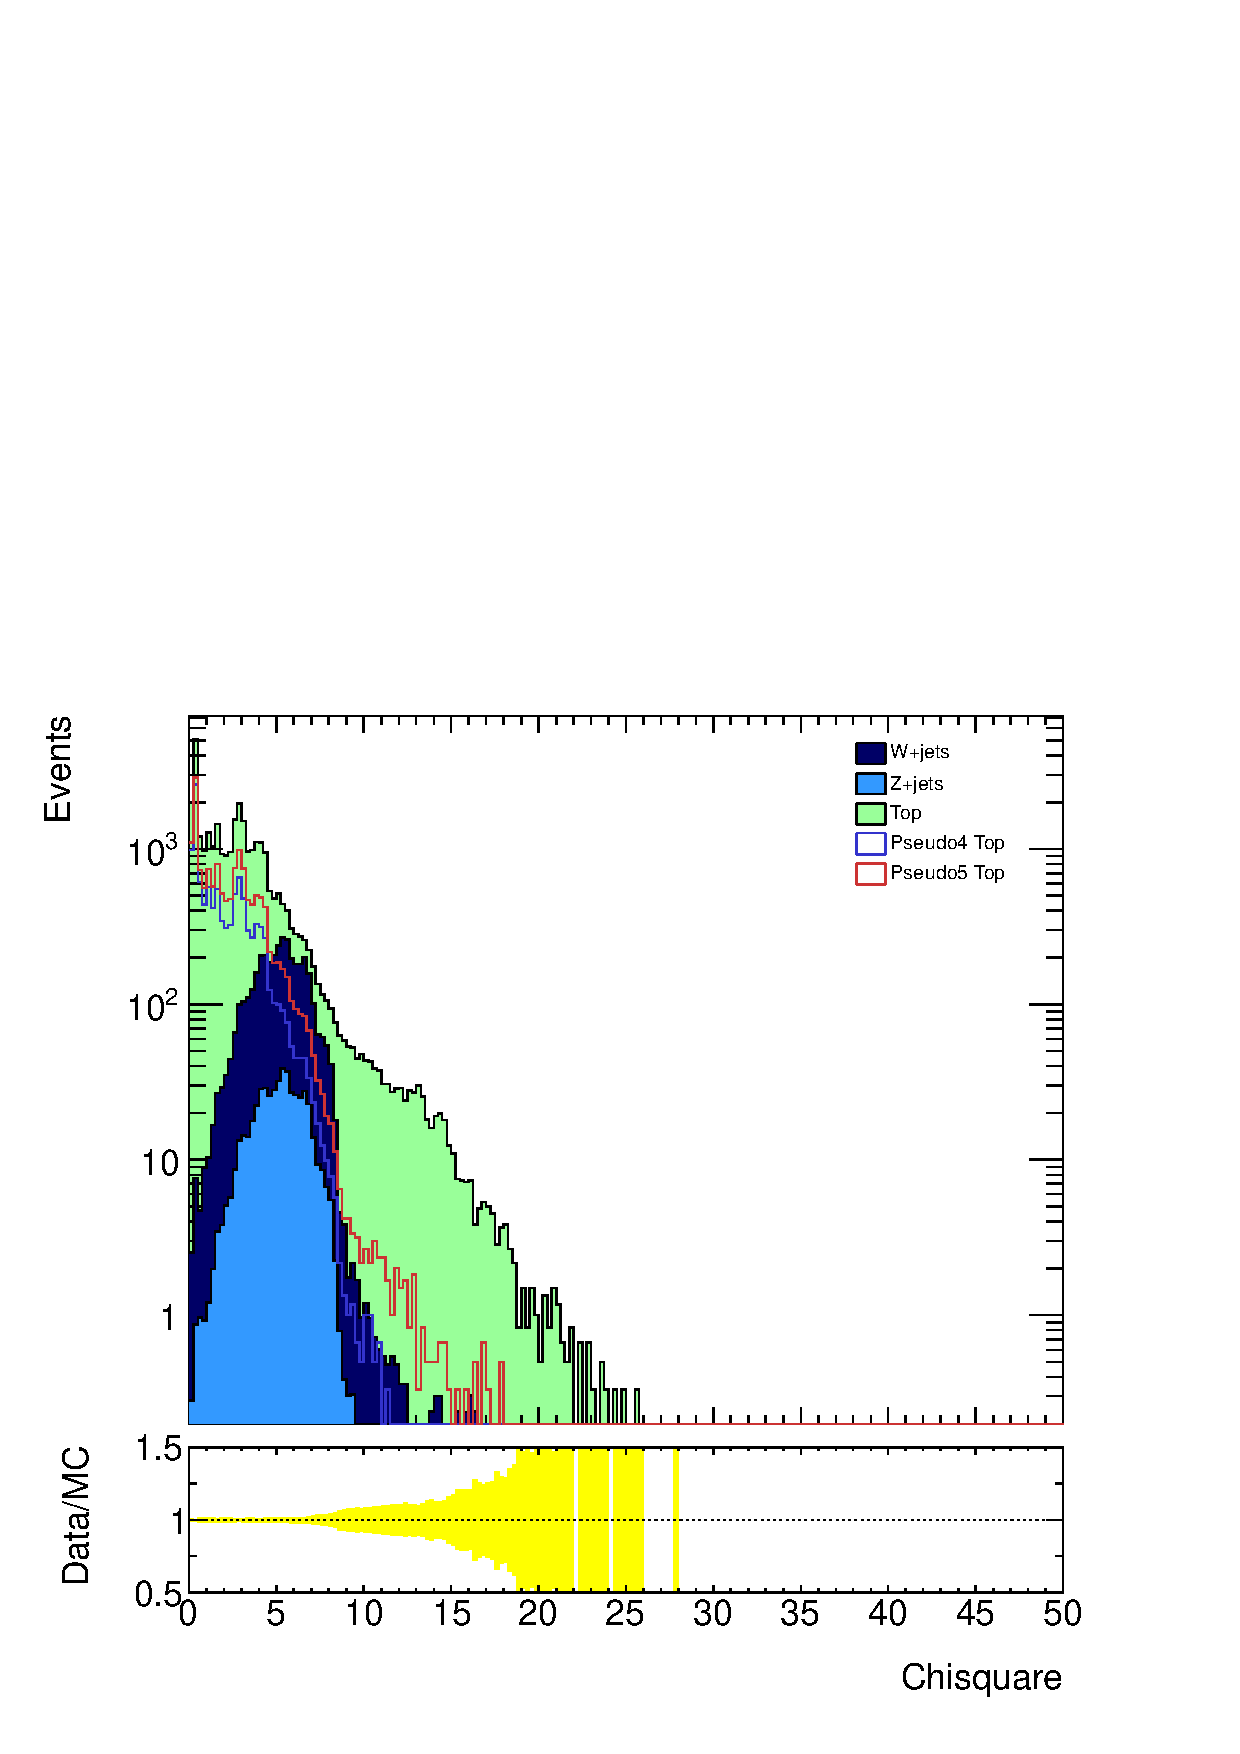
\includegraphics[scale=0.275]{img/Total__min_chi_kin_all4.pdf}
    \end{figure}\end{column}
    \begin{column}{0.45\textwidth}\begin{figure}
      \caption{$\chi^2_{B}$}
      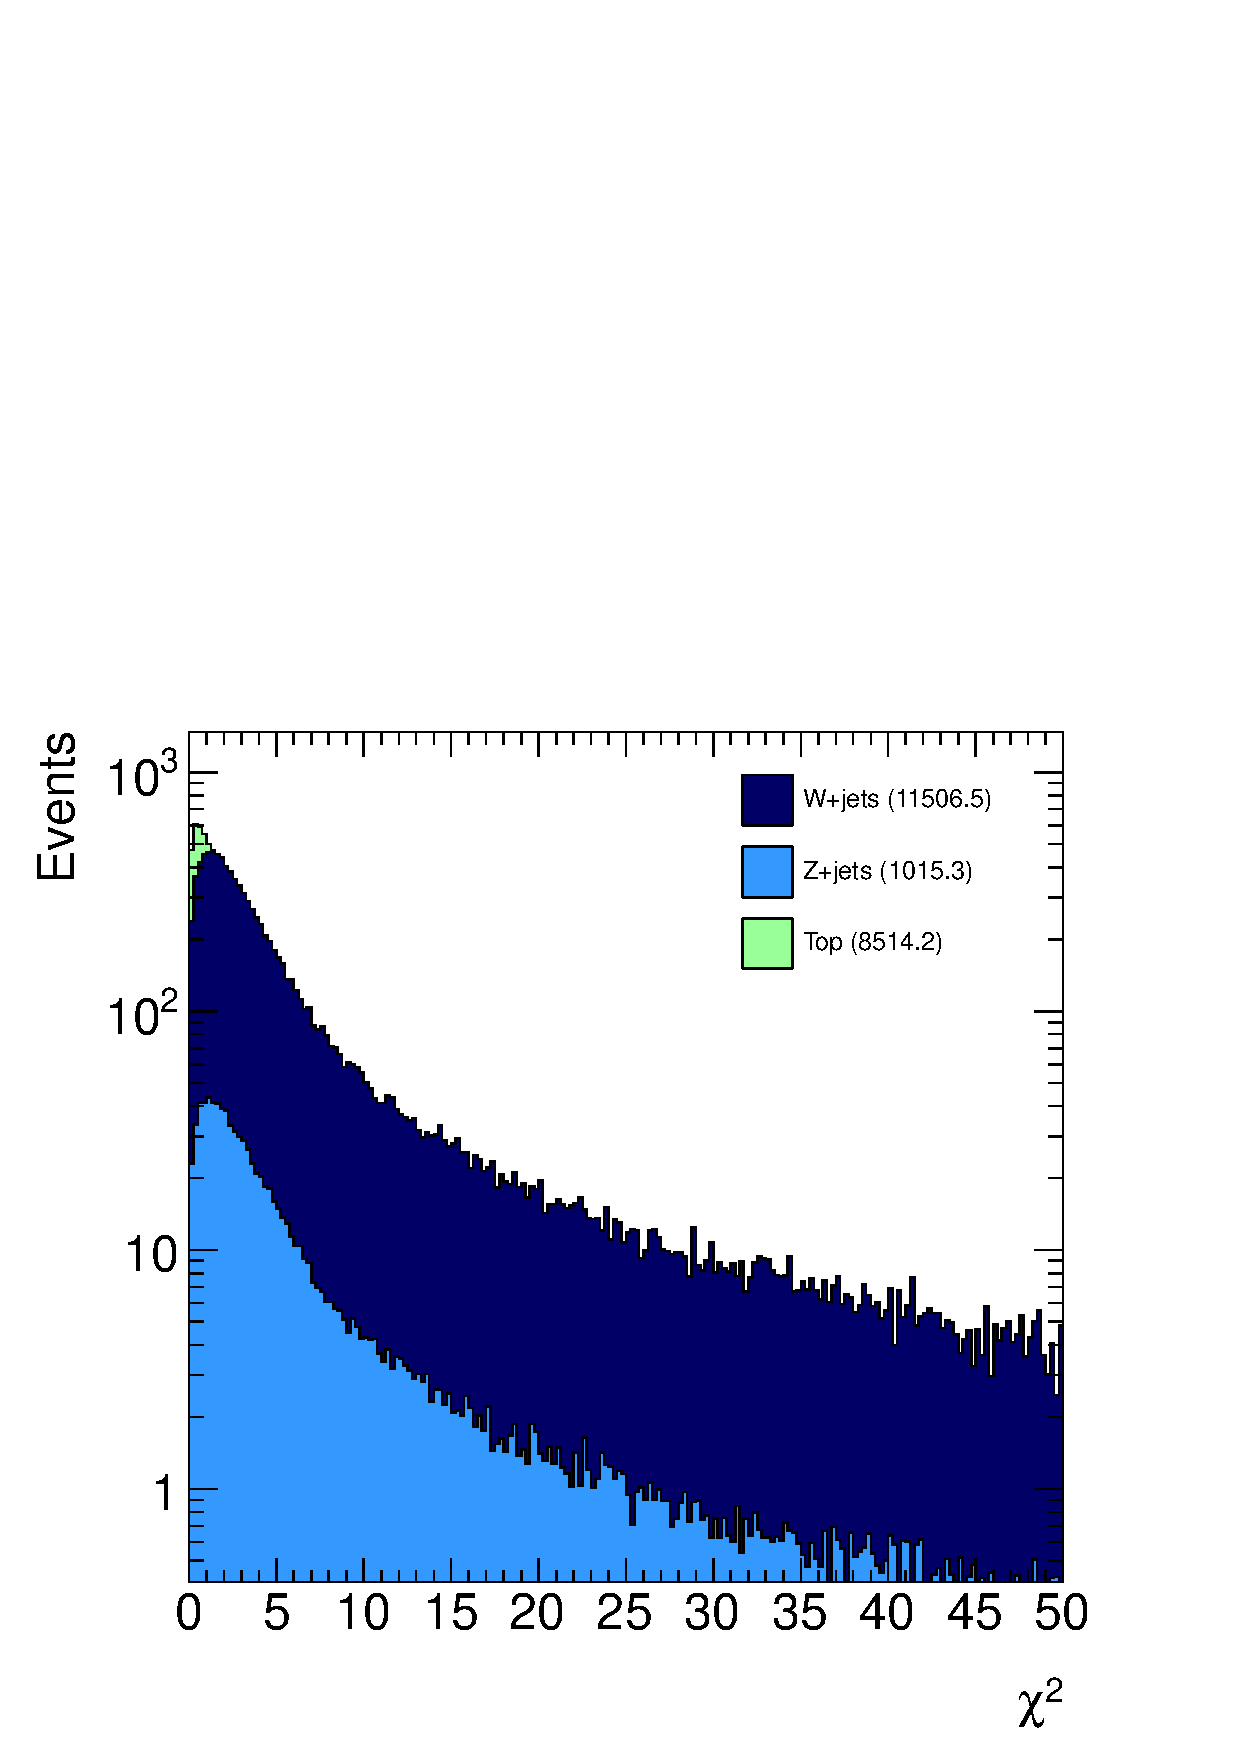
\includegraphics[scale=0.275]{img/Total__min_chi_B_all4.pdf}
    \end{figure}\end{column}
  \end{columns}
\end{frame}

\begin{frame}{Total Chisquare distribution}
  \begin{columns}
    \begin{column}{0.45\textwidth}\begin{figure}
      \caption{$\chi^2$ = $\chi^2_{kinematic} + \chi^2_{B}$}
      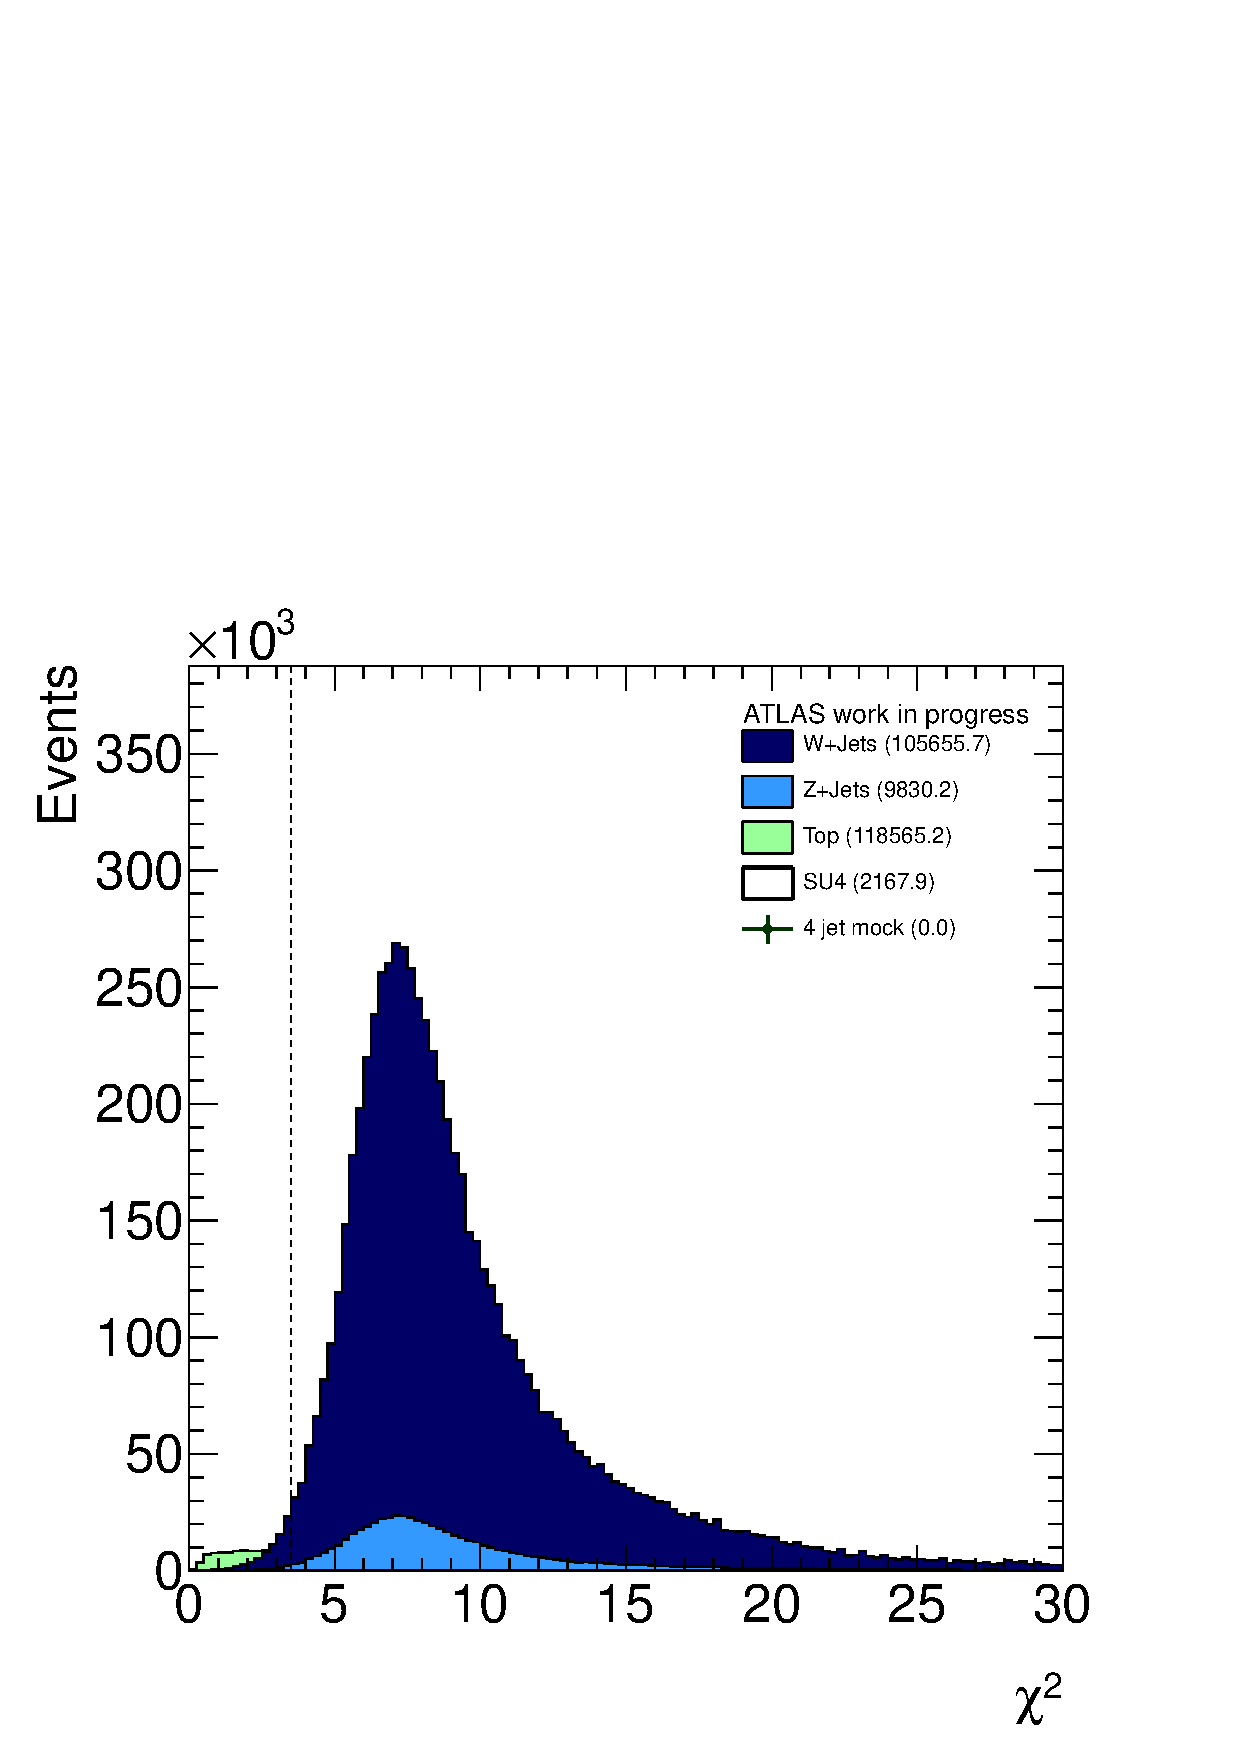
\includegraphics[scale=0.275]{img/Total__min_chi_all_all4.pdf}
    \end{figure}\end{column}
  \end{columns}
\end{frame}

\begin{frame}
Using the $\chi^2$ as a descriminate alone gives $t\bar{t}$ purity $\approx80\%$ in $t\bar{t}$ samples where all decay products are reconstructed.

Total $t\bar{t}$ purity including backgrounds is $\mathcal{O}\left(60\%\right)$.

Further descrimination may be obtained by looking at likelihoods for the event maps.

\end{frame}

\begin{frame}
We can form a probability of correct assignment, using the likelihood for a correct map;
  \begin{equation}\begin{split}
    L\left(a,b,c,d\right) =&
    \frac{1}{\sqrt{2\pi}\sigma_{W_{h}}} \exp^{-\left(m_{ab}-M_{W}\right)^{2} / 2\sigma^{2}_{W_{h}}}
    \frac{1}{\sqrt{2\pi}\sigma_{t_{h}}} \exp^{-\left(m_{abc}-m_{t}\right)^{2} / 2\sigma^{2}_{t_{h}}}
    \\&\times
    \frac{1}{\sqrt{2\pi}\sigma_{W_{l}}} \exp^{-\left(m_{dl\nu}-m_{t}\right)^{2} / 2\sigma^{2}_{t_{l}}}
    \\&\times
    L_{W}\left(\omega_{a},\omega_{b}\right) L_{bb}\left(\omega_{c},\omega_{d}\right),
  \end{split}\end{equation}
by summing all likelihoods where jets $a$ \& $b$ are assigned to the hadronic W.
\begin{equation}
P_{CA} = \frac{L\left(a,b,c,d\right) + L\left(a,b,d,c\right) + L\left(b,a,c,d\right) + L\left(b,a,d,c\right)}{\sum_{\text{all maps}} L\left(\text{map}\right)}
\end{equation}
\end{frame}

\section{Performance}

\begin{frame}{Jet pT}
  \begin{columns}
    \begin{column}{0.45\textwidth}\begin{figure}
      \caption{$e^{+}e^{-}$$p_{T}^{\text{jet 1}}$}
      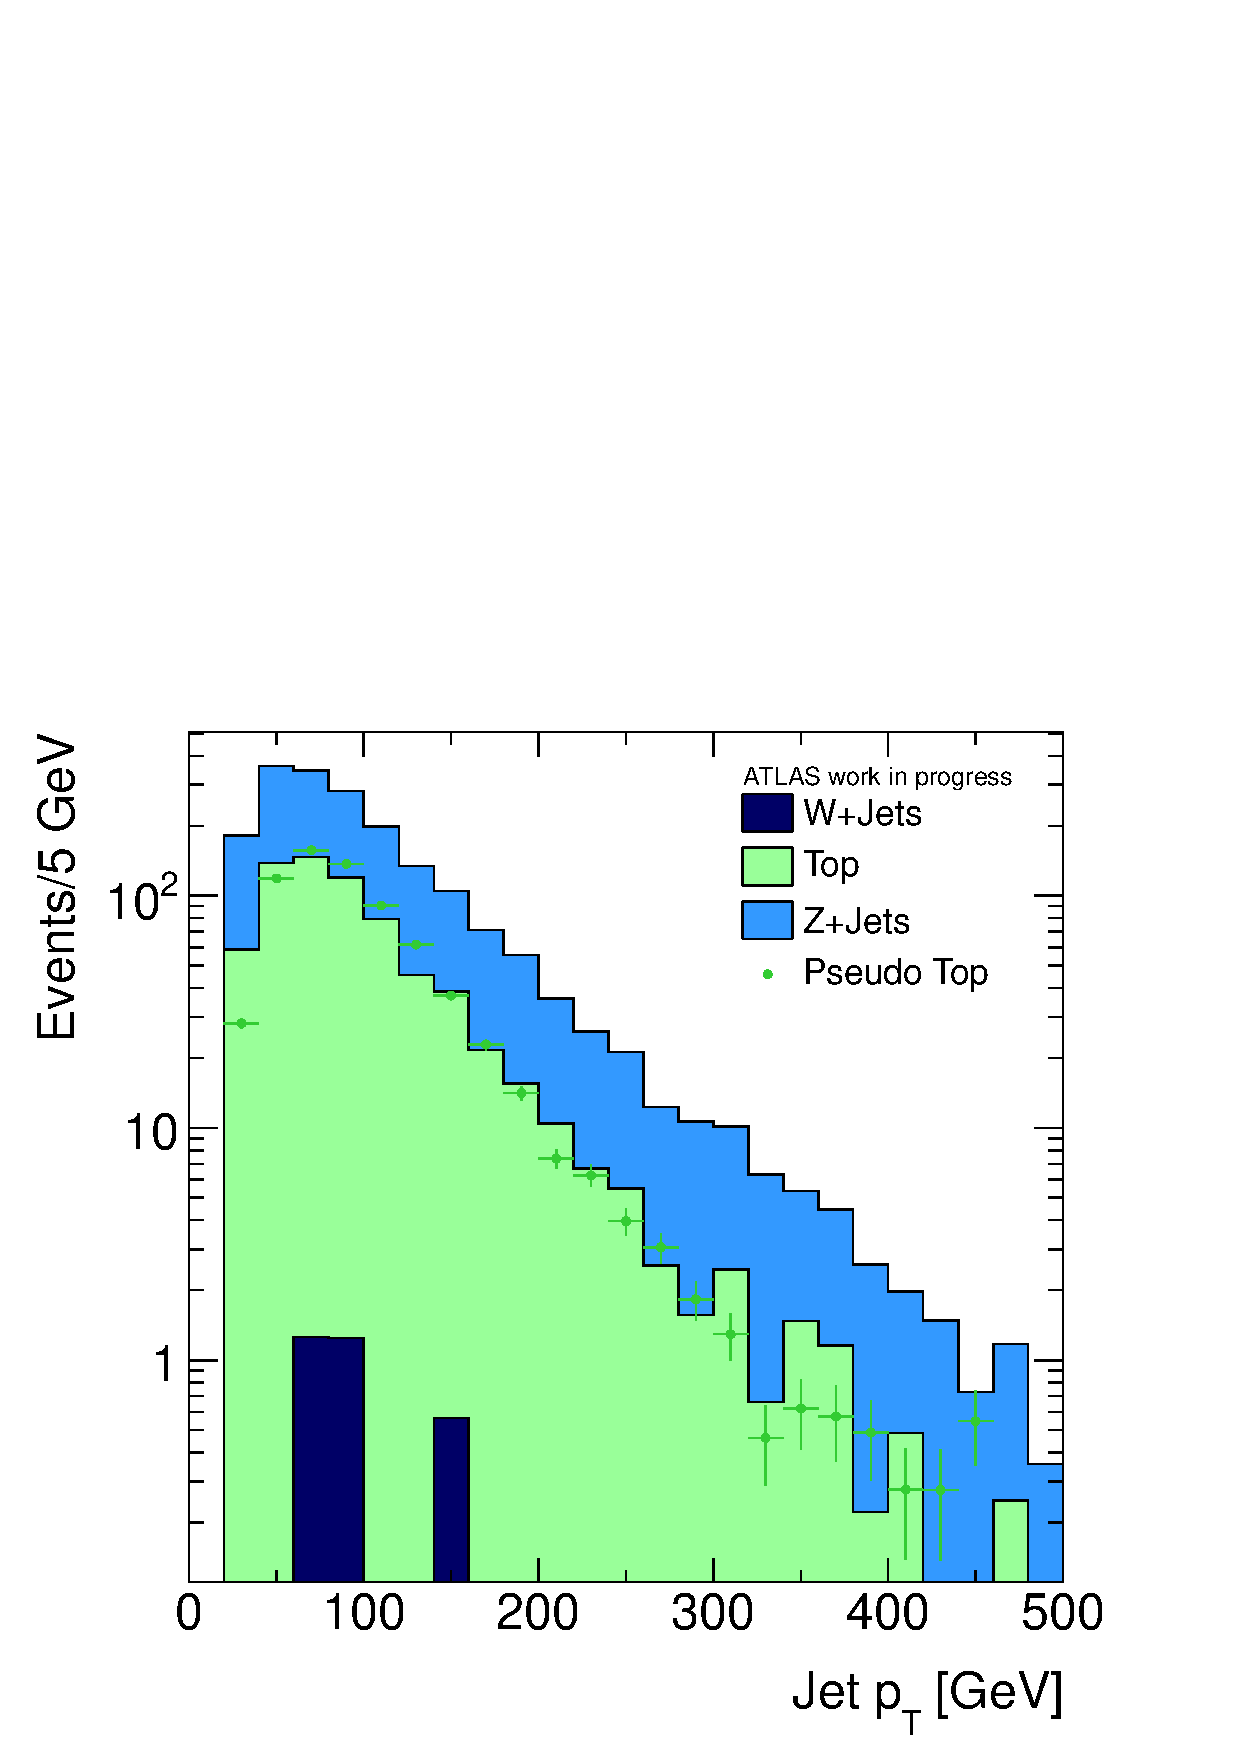
\includegraphics[scale=0.275]{img/Total_OS_EE_jet_lead_pt_scaled.pdf}
    \end{figure}\end{column}
    \begin{column}{0.45\textwidth}\begin{figure}
      \caption{$e^{+}e^{-}$$p_{T}^{\text{jet 2}}$}
      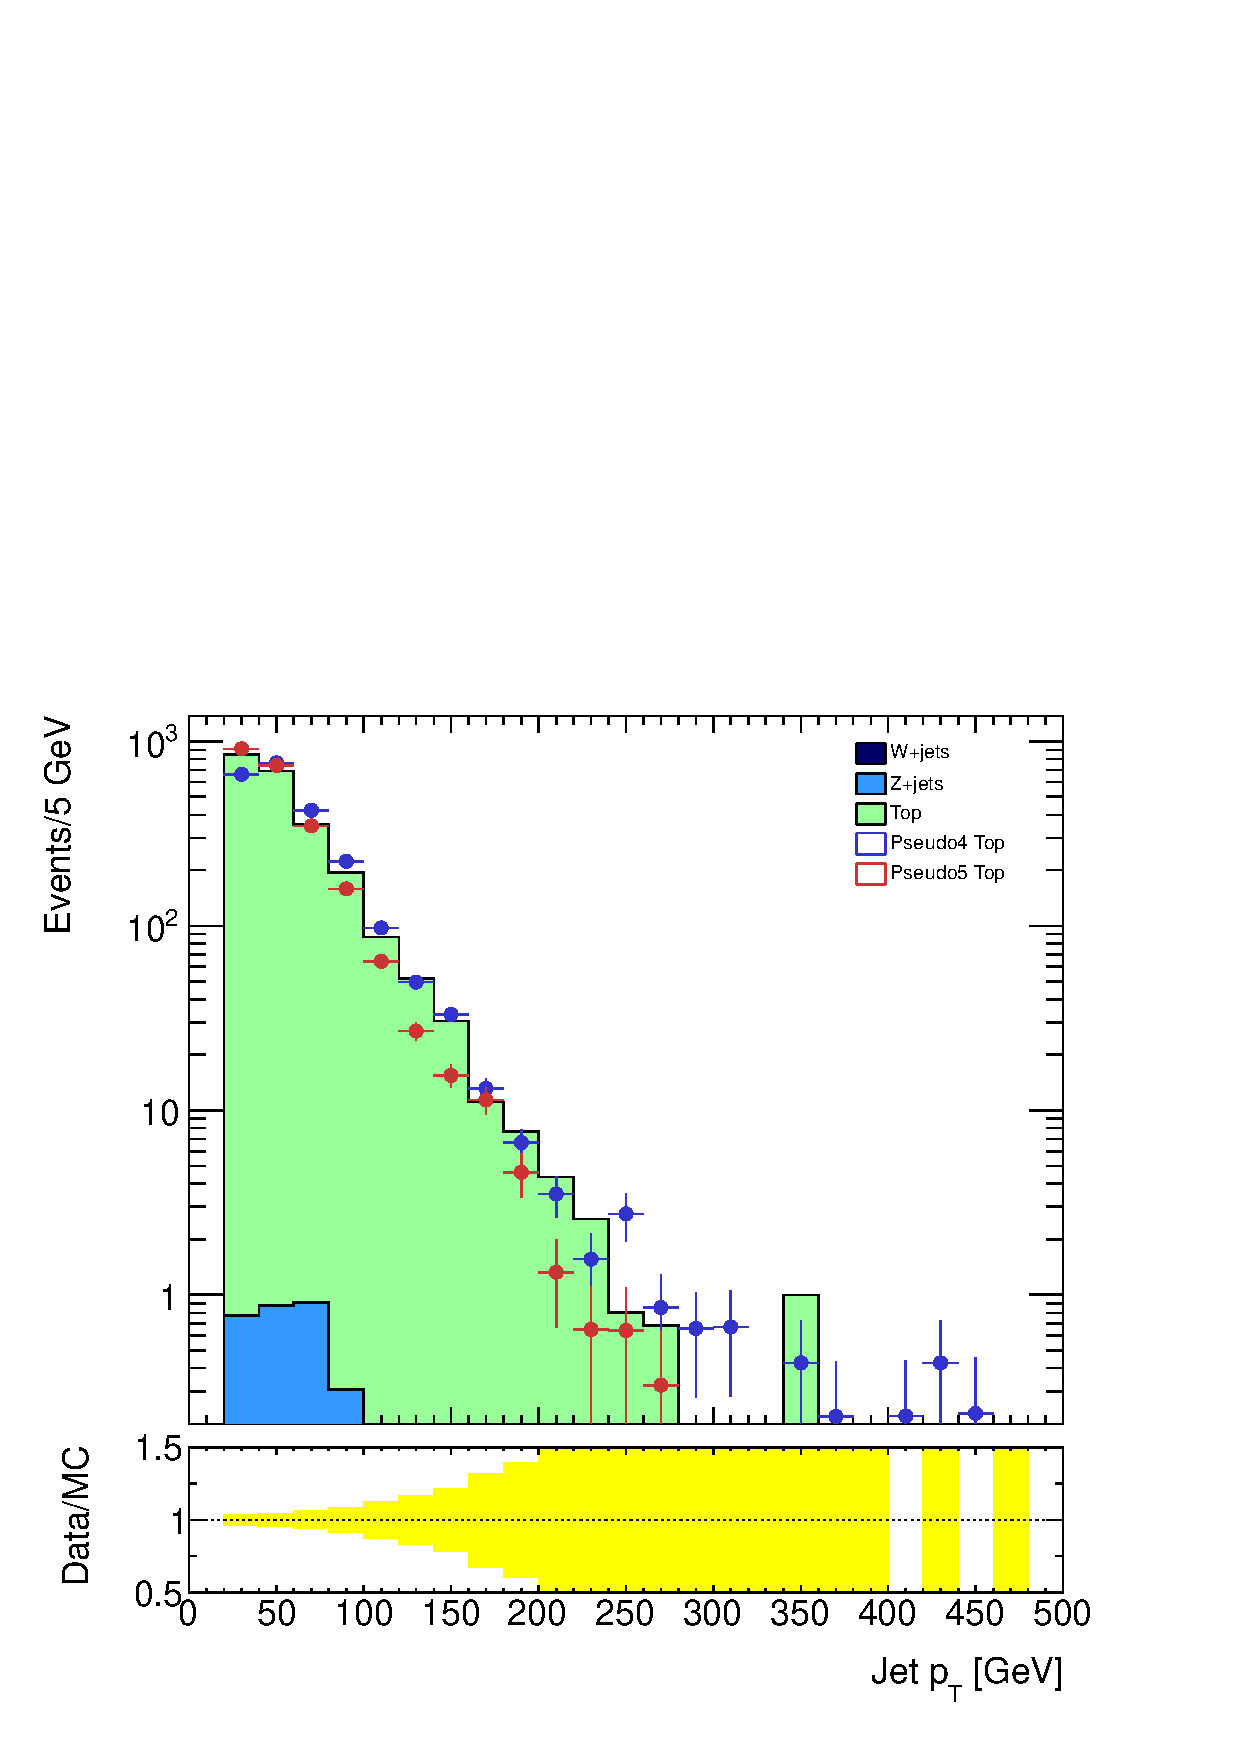
\includegraphics[scale=0.275]{img/Total_OS_EE_jet_lead2_pt_scaled.pdf}
    \end{figure}\end{column}
  \end{columns}
\end{frame}

\begin{frame}{Effective mass}
  \begin{columns}
    \begin{column}{0.45\textwidth}\begin{figure}
      \caption{$e^{+}e^{-}$$\slashed{E}_{T}$}
      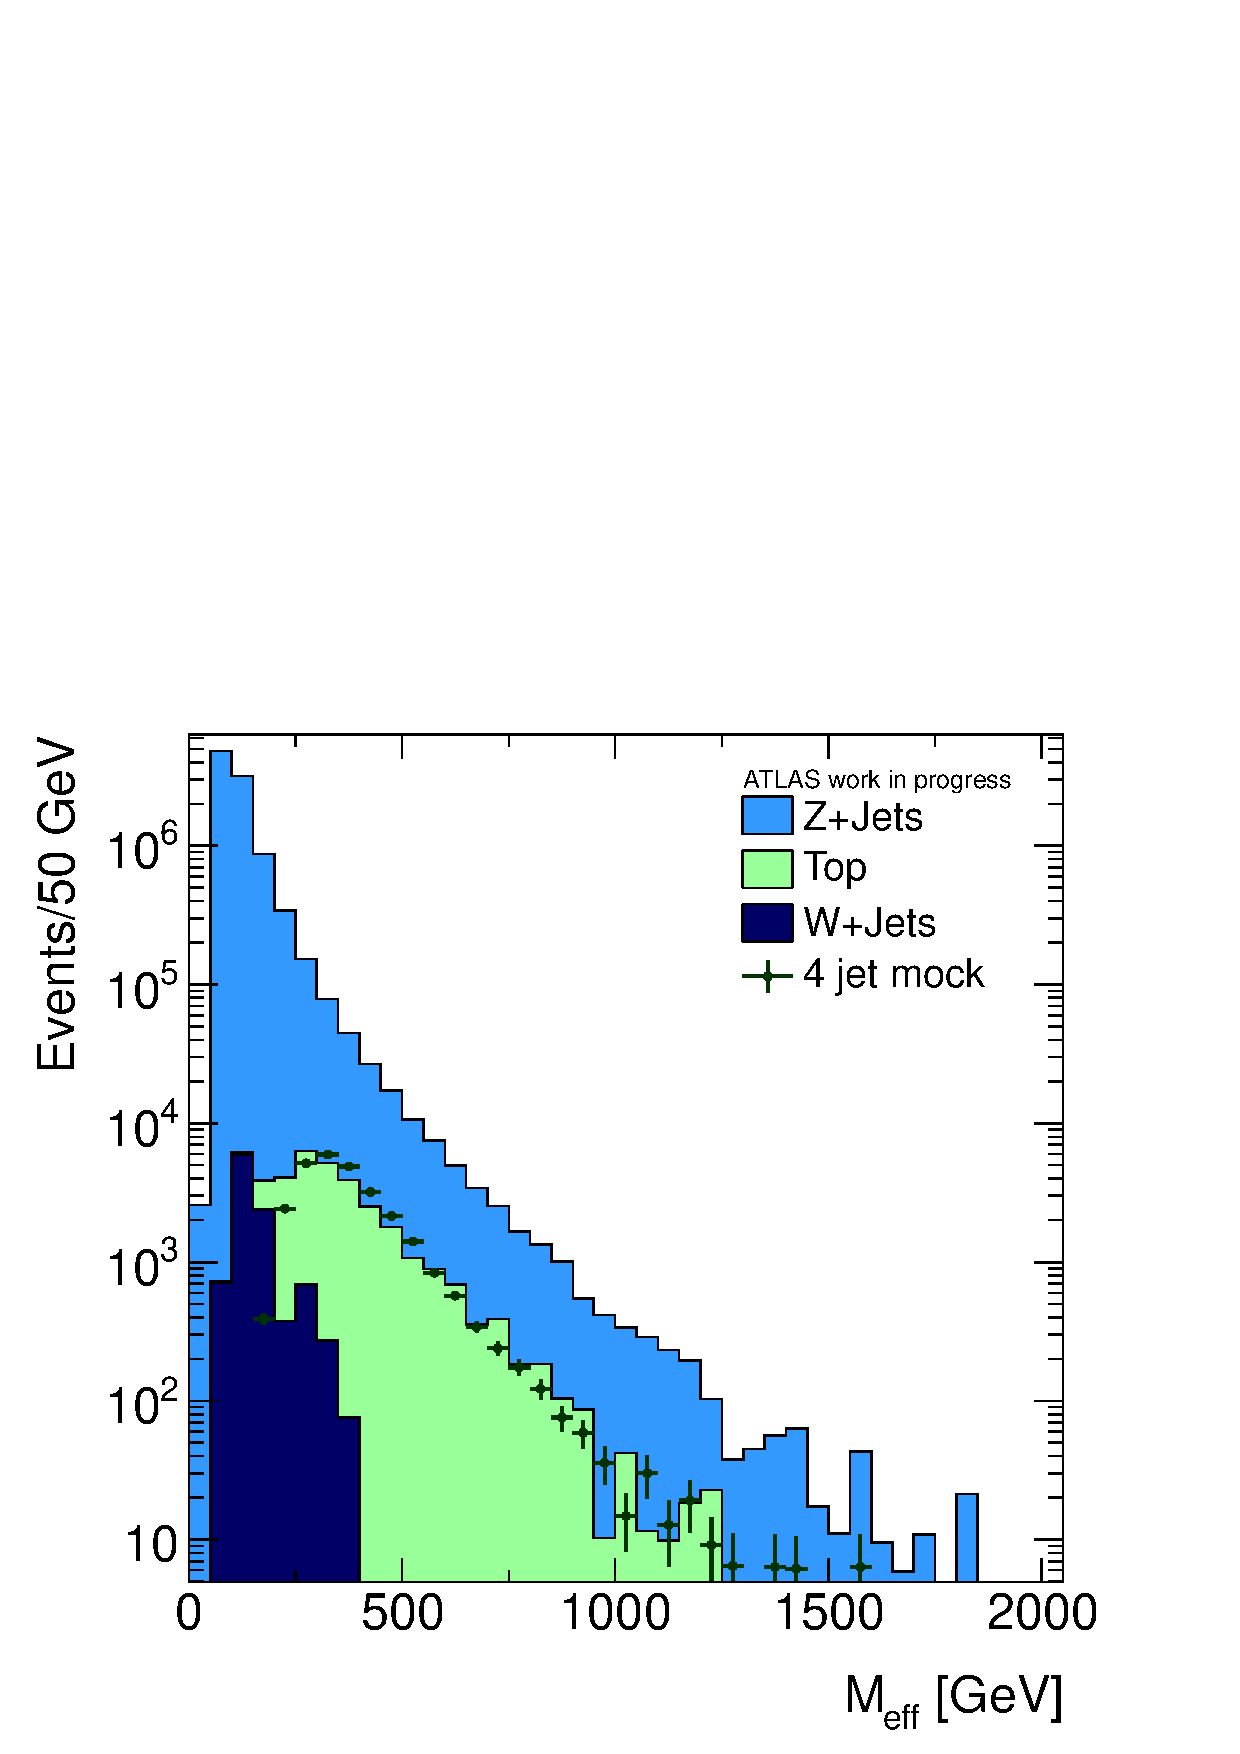
\includegraphics[scale=0.275]{img/Total_OS_EE_meff_scaled.pdf}
    \end{figure}\end{column}
    \begin{column}{0.45\textwidth}\begin{figure}
      \caption{$\mu^{+}\mu^{-}$$\slashed{E}_{T}$}
      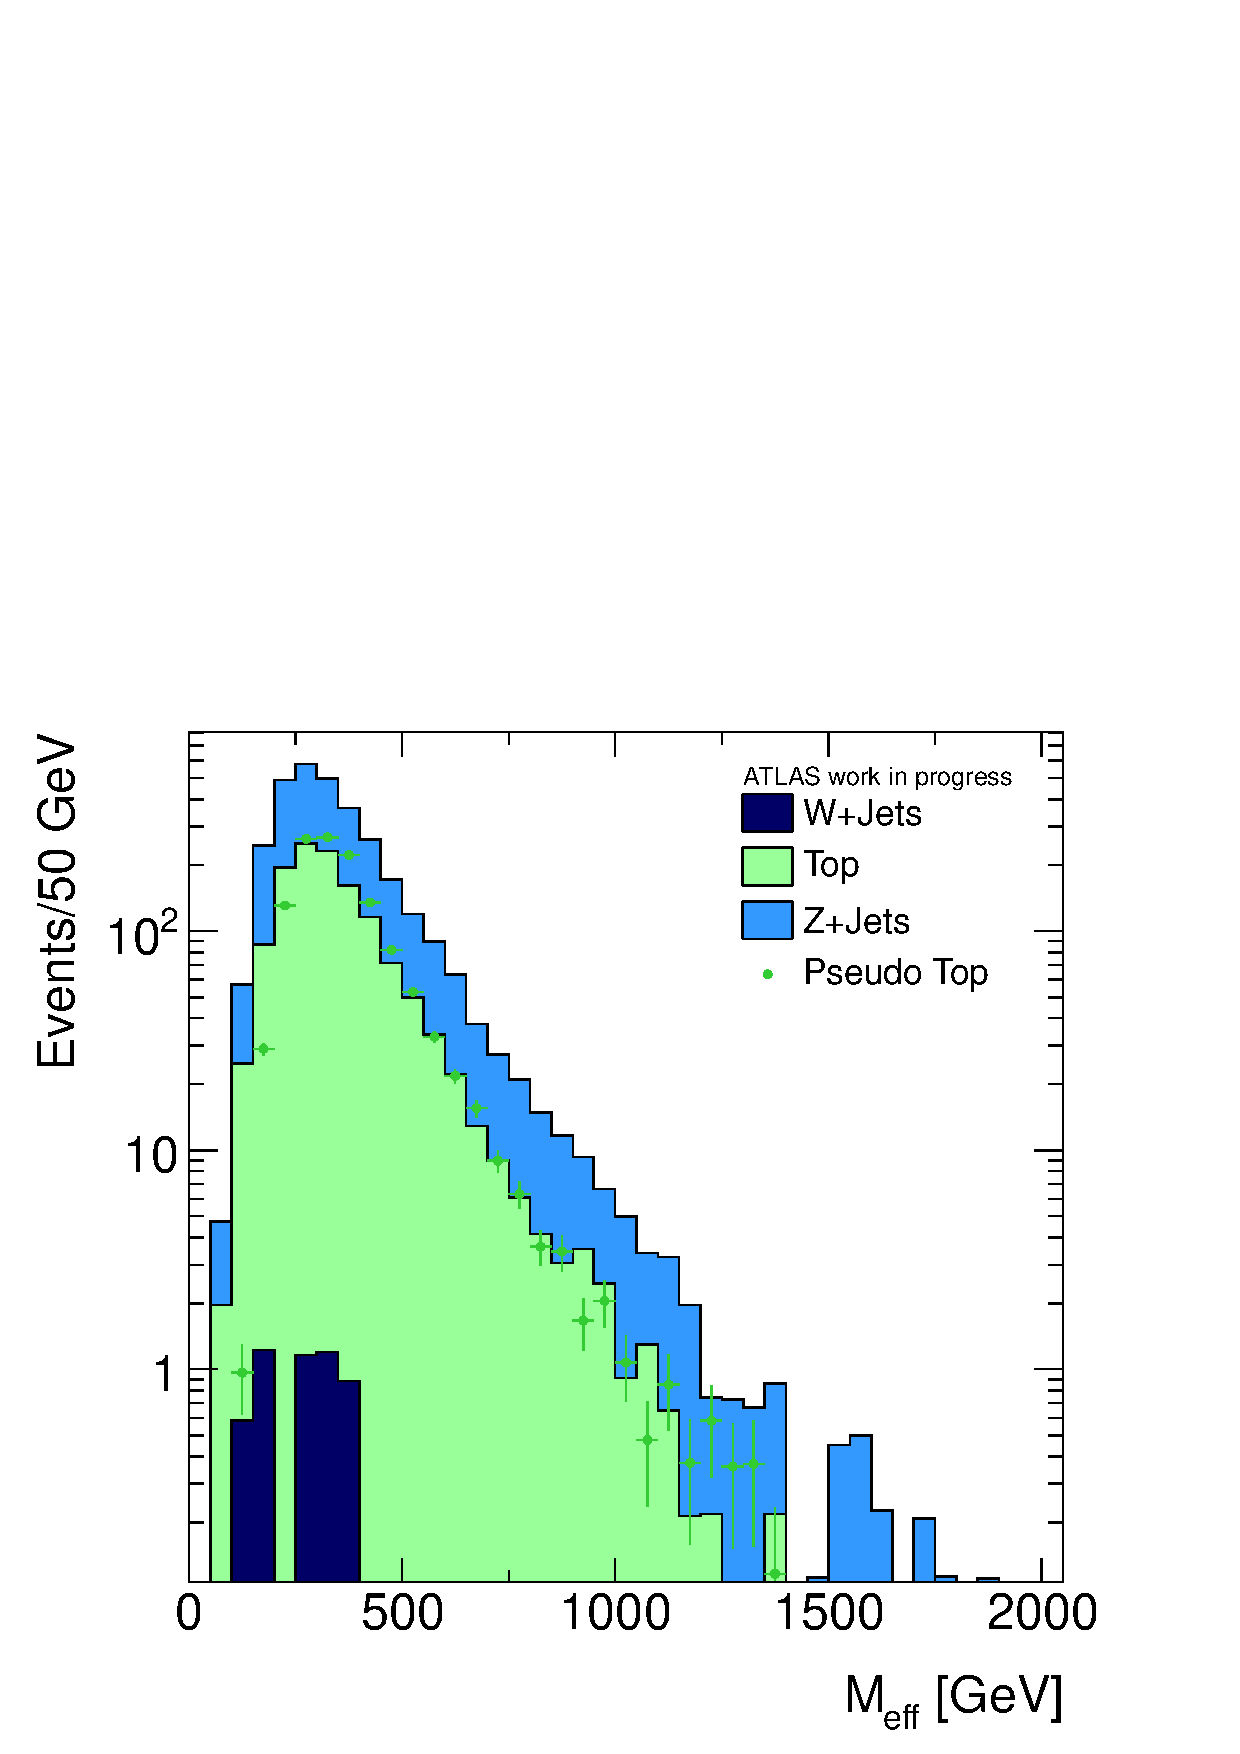
\includegraphics[scale=0.275]{img/Total_OS_MM_meff_scaled.pdf}
    \end{figure}\end{column}
  \end{columns}
\end{frame}

\begin{frame}{Missing ET}
  \begin{columns}
    \begin{column}{0.45\textwidth}\begin{figure}
      \caption{$e^{+}e^{-}$$\slashed{E}_{T}$}
      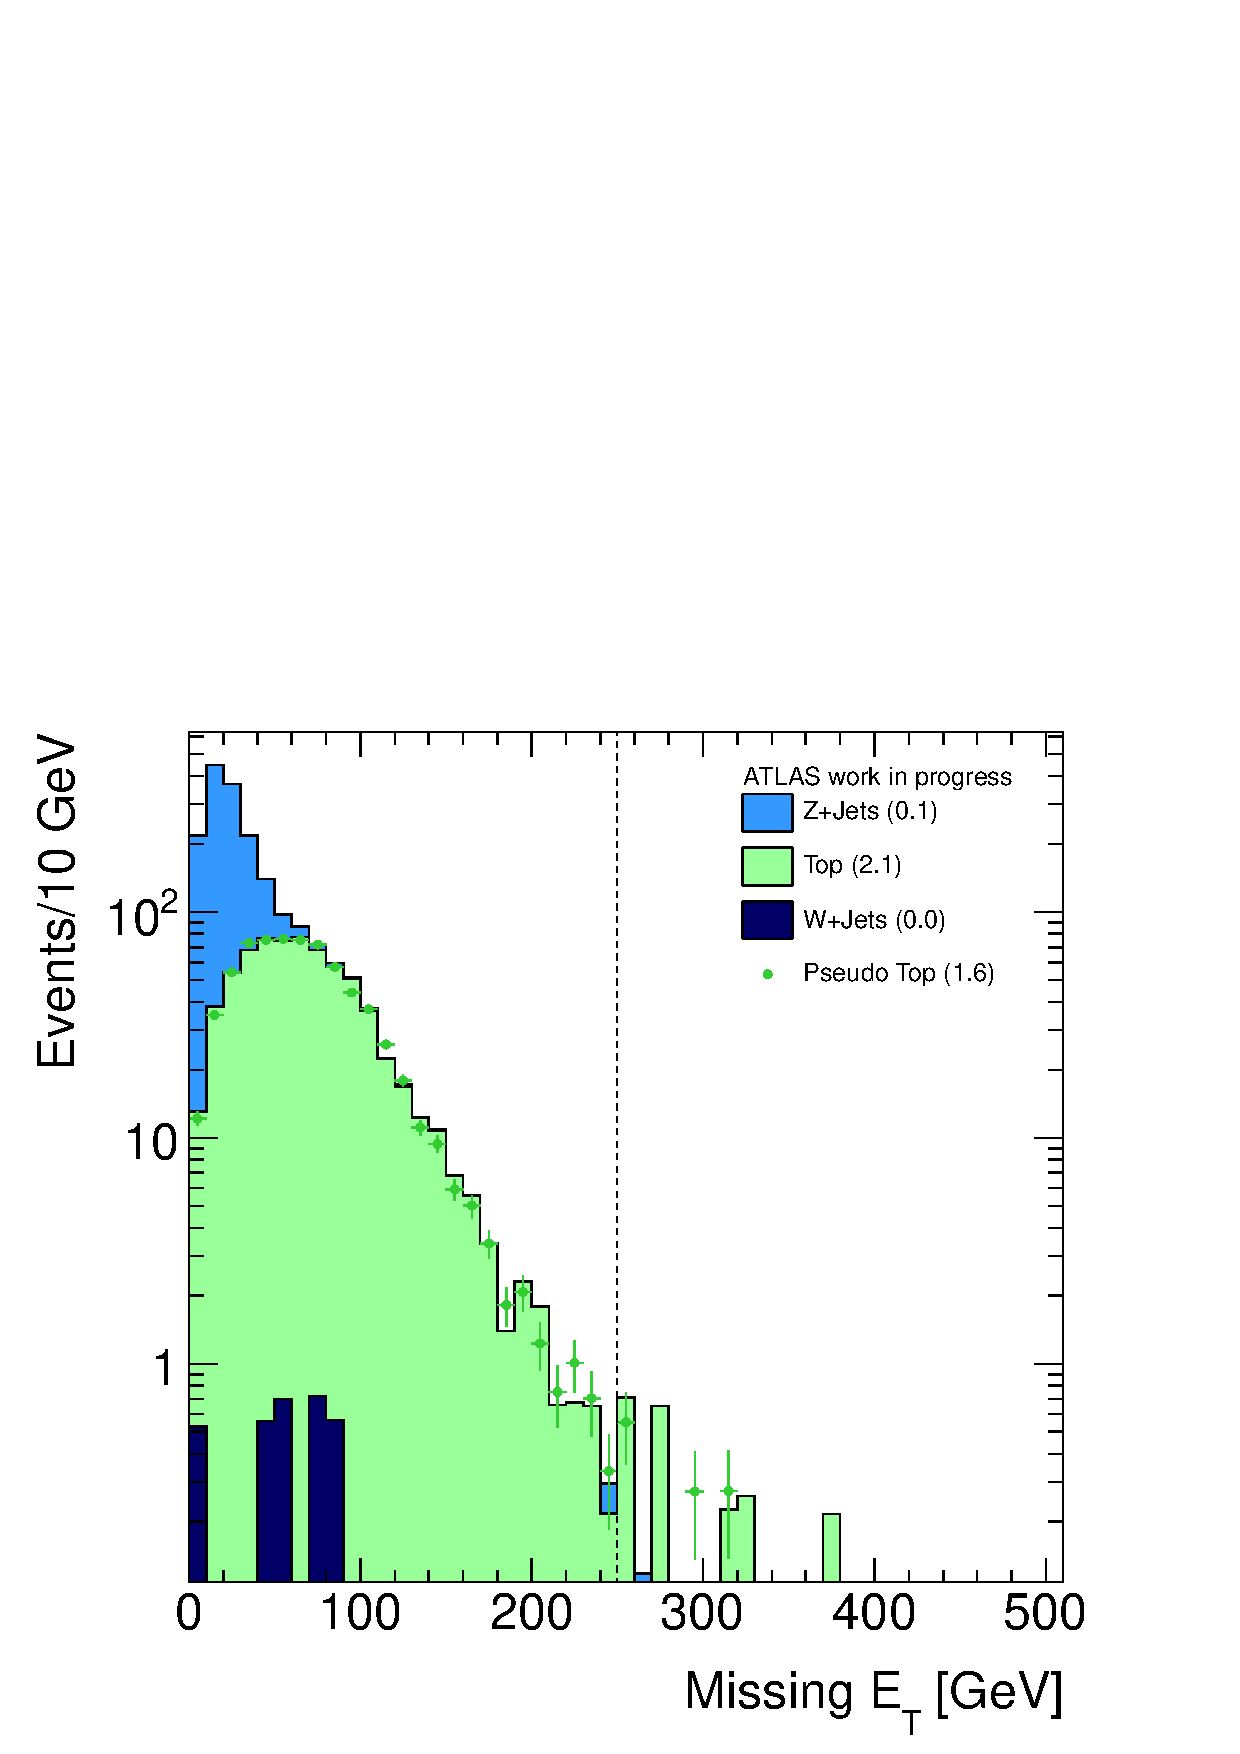
\includegraphics[scale=0.275]{img/Total_OS_EE_etmiss_scaled.pdf}
    \end{figure}\end{column}
    \begin{column}{0.45\textwidth}\begin{figure}
      \caption{$\mu^{+}\mu^{-}$$\slashed{E}_{T}$}
      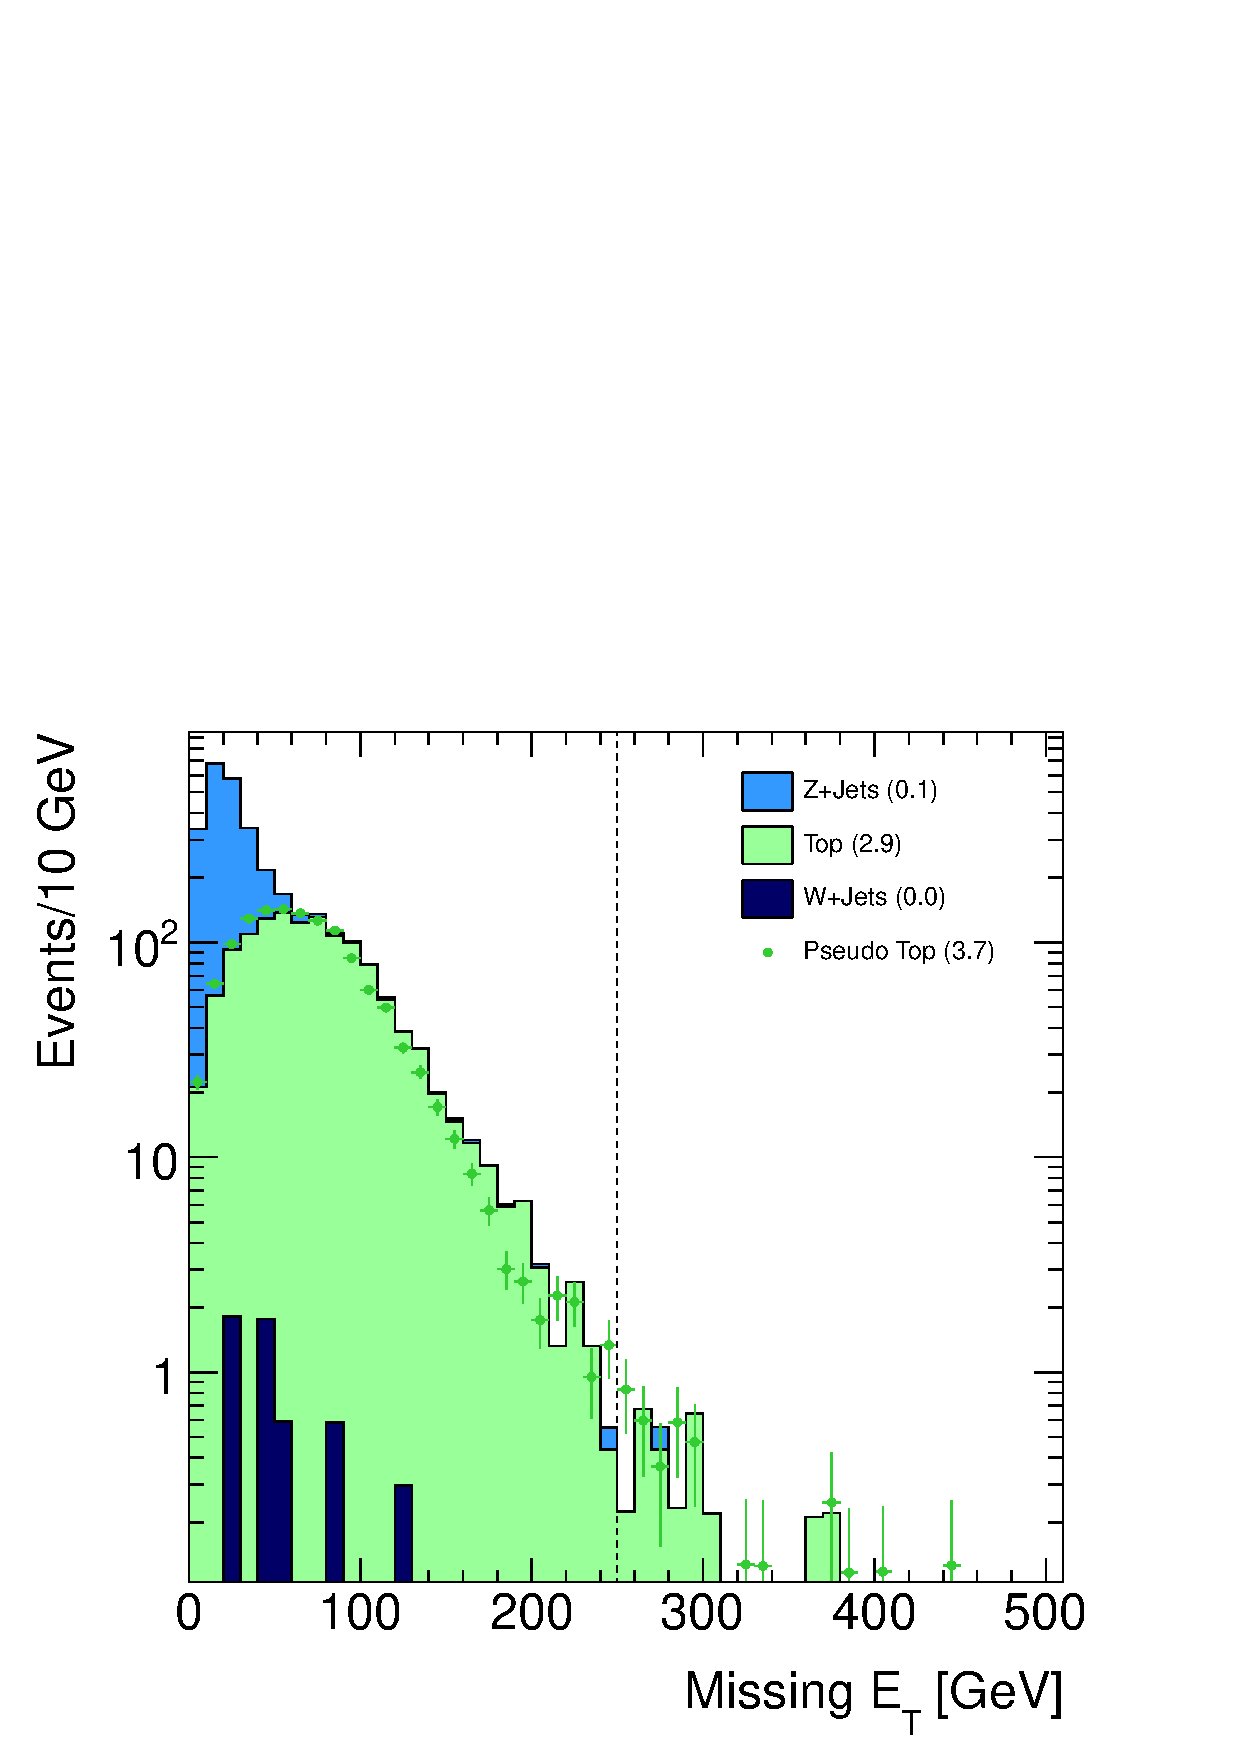
\includegraphics[scale=0.275]{img/Total_OS_MM_etmiss_scaled.pdf}
    \end{figure}\end{column}
  \end{columns}
\end{frame}

\begin{frame}{Further work}
  \begin{itemize}
    \item Optimise cuts on $\chi^2$ and correct assignment probabilities.
    \item Futher develop $1\text{l}+5\text{j}$ control for $2\text{l}+3\text{j}$ search.
    \item Run through full statistical analysis of technique.
  \end{itemize}
\end{frame}

\begin{frame}{Thanks}
  MC event graphs rendered with MCViz (\url{MCViz.net}).
\end{frame}

\begin{frame}{Effective mass - different flavour}
  \begin{columns}
    \begin{column}{0.45\textwidth}\begin{figure}
      \caption{$e^{\pm}\mu^{\mp}$$\slashed{E}_{T}$}
      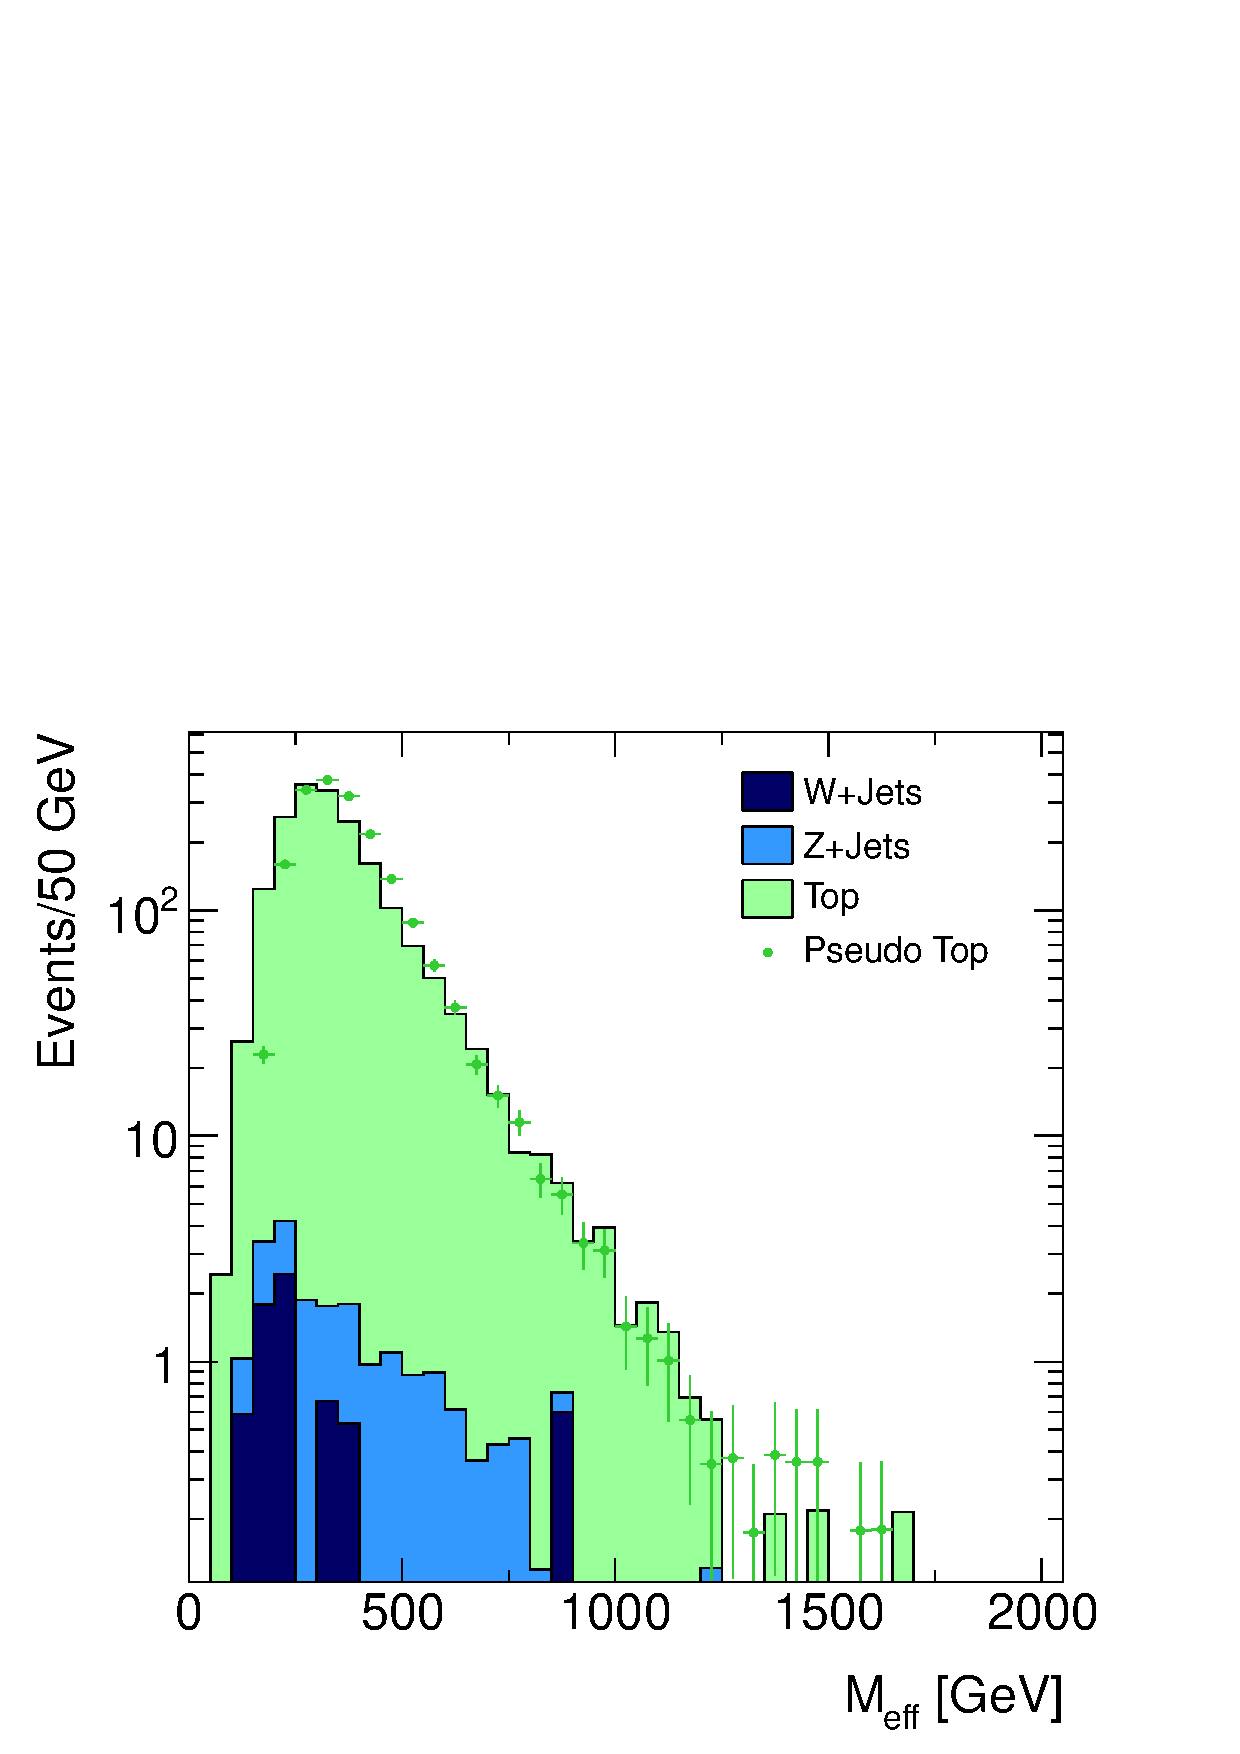
\includegraphics[scale=0.275]{img/Total_OS_EM_meff_scaled.pdf}
    \end{figure}\end{column}
    \begin{column}{0.45\textwidth}\begin{figure}
      \caption{$\mu^{\pm}e^{\mp}$$\slashed{E}_{T}$}
      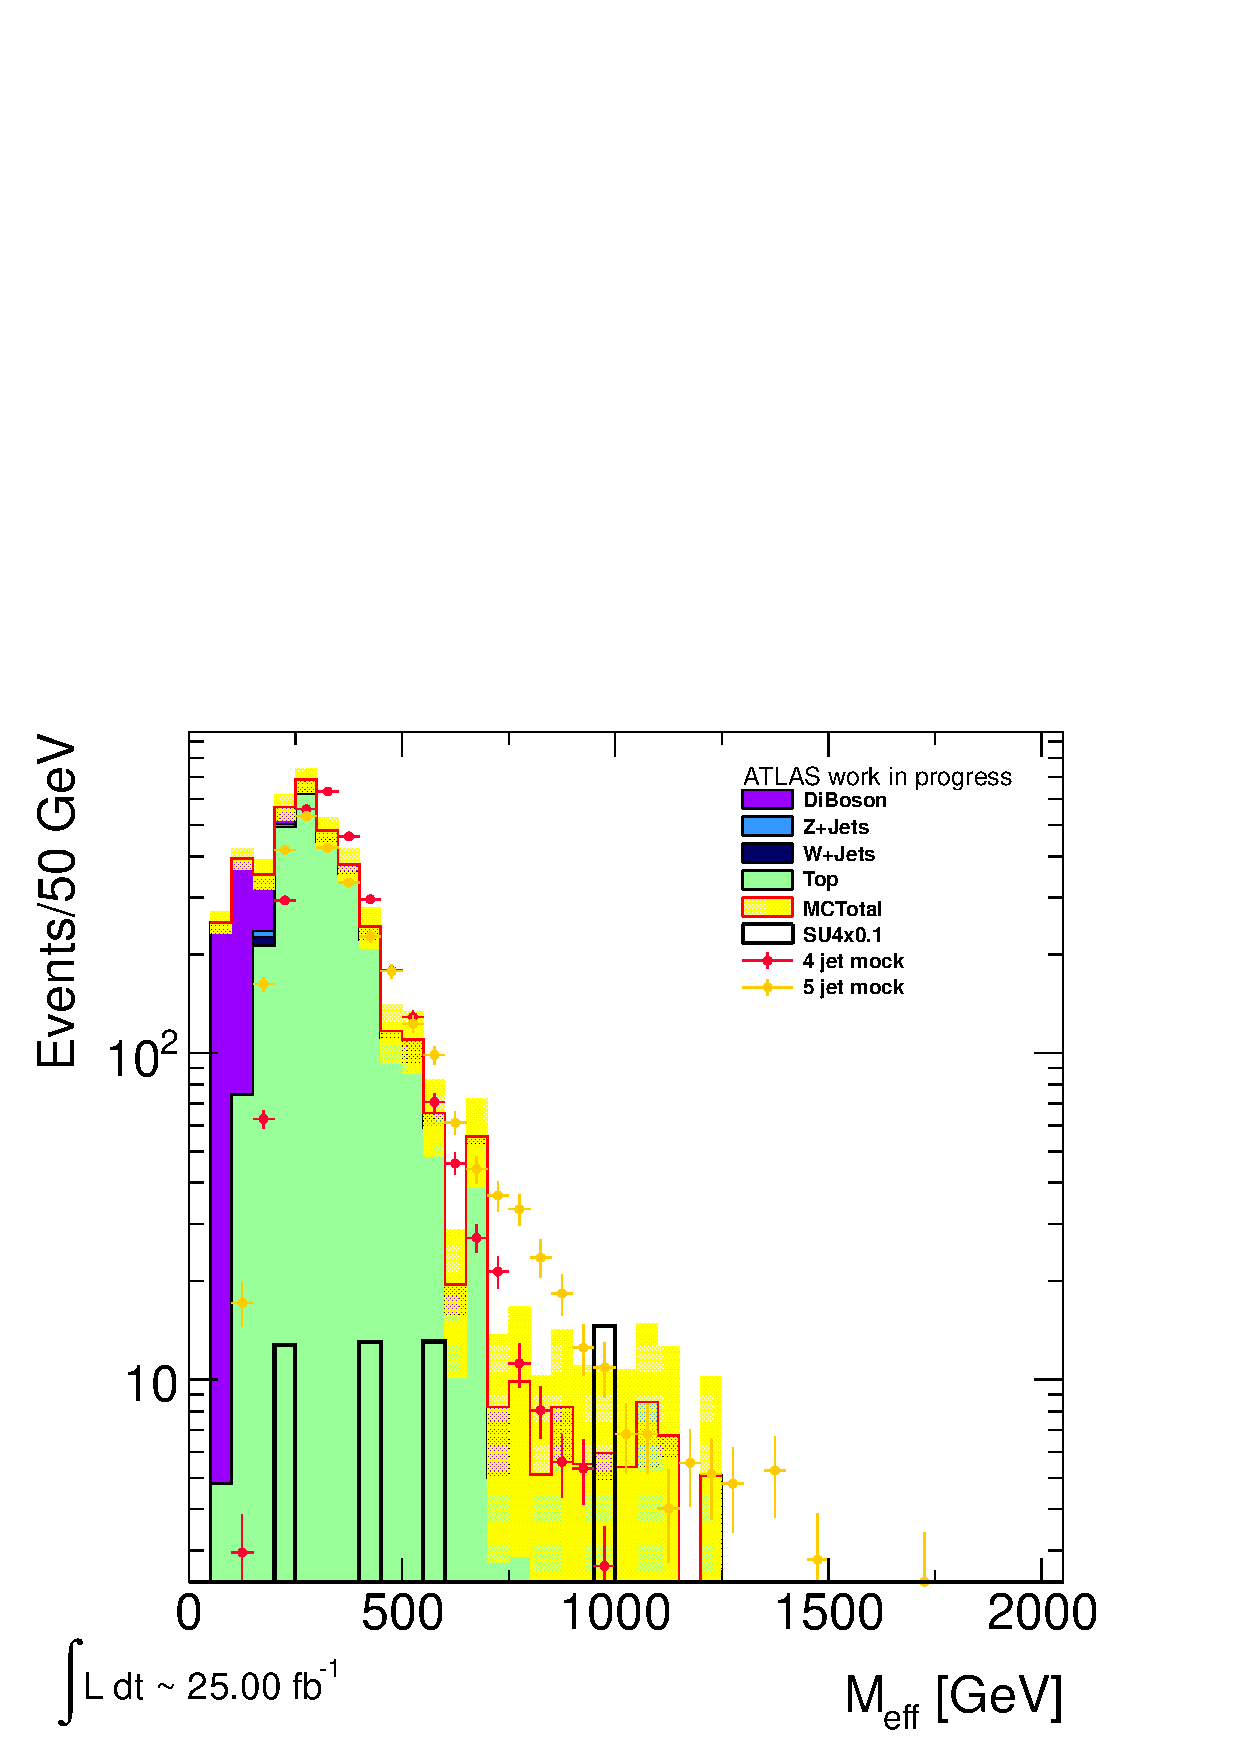
\includegraphics[scale=0.275]{img/Total_OS_ME_meff_scaled.pdf}
    \end{figure}\end{column}
  \end{columns}
\end{frame}

\begin{frame}{Missing ET - different flavour}
  \begin{columns}
    \begin{column}{0.45\textwidth}\begin{figure}
      \caption{$e^{\pm}\mu^{\mp}$$\slashed{E}_{T}$}
      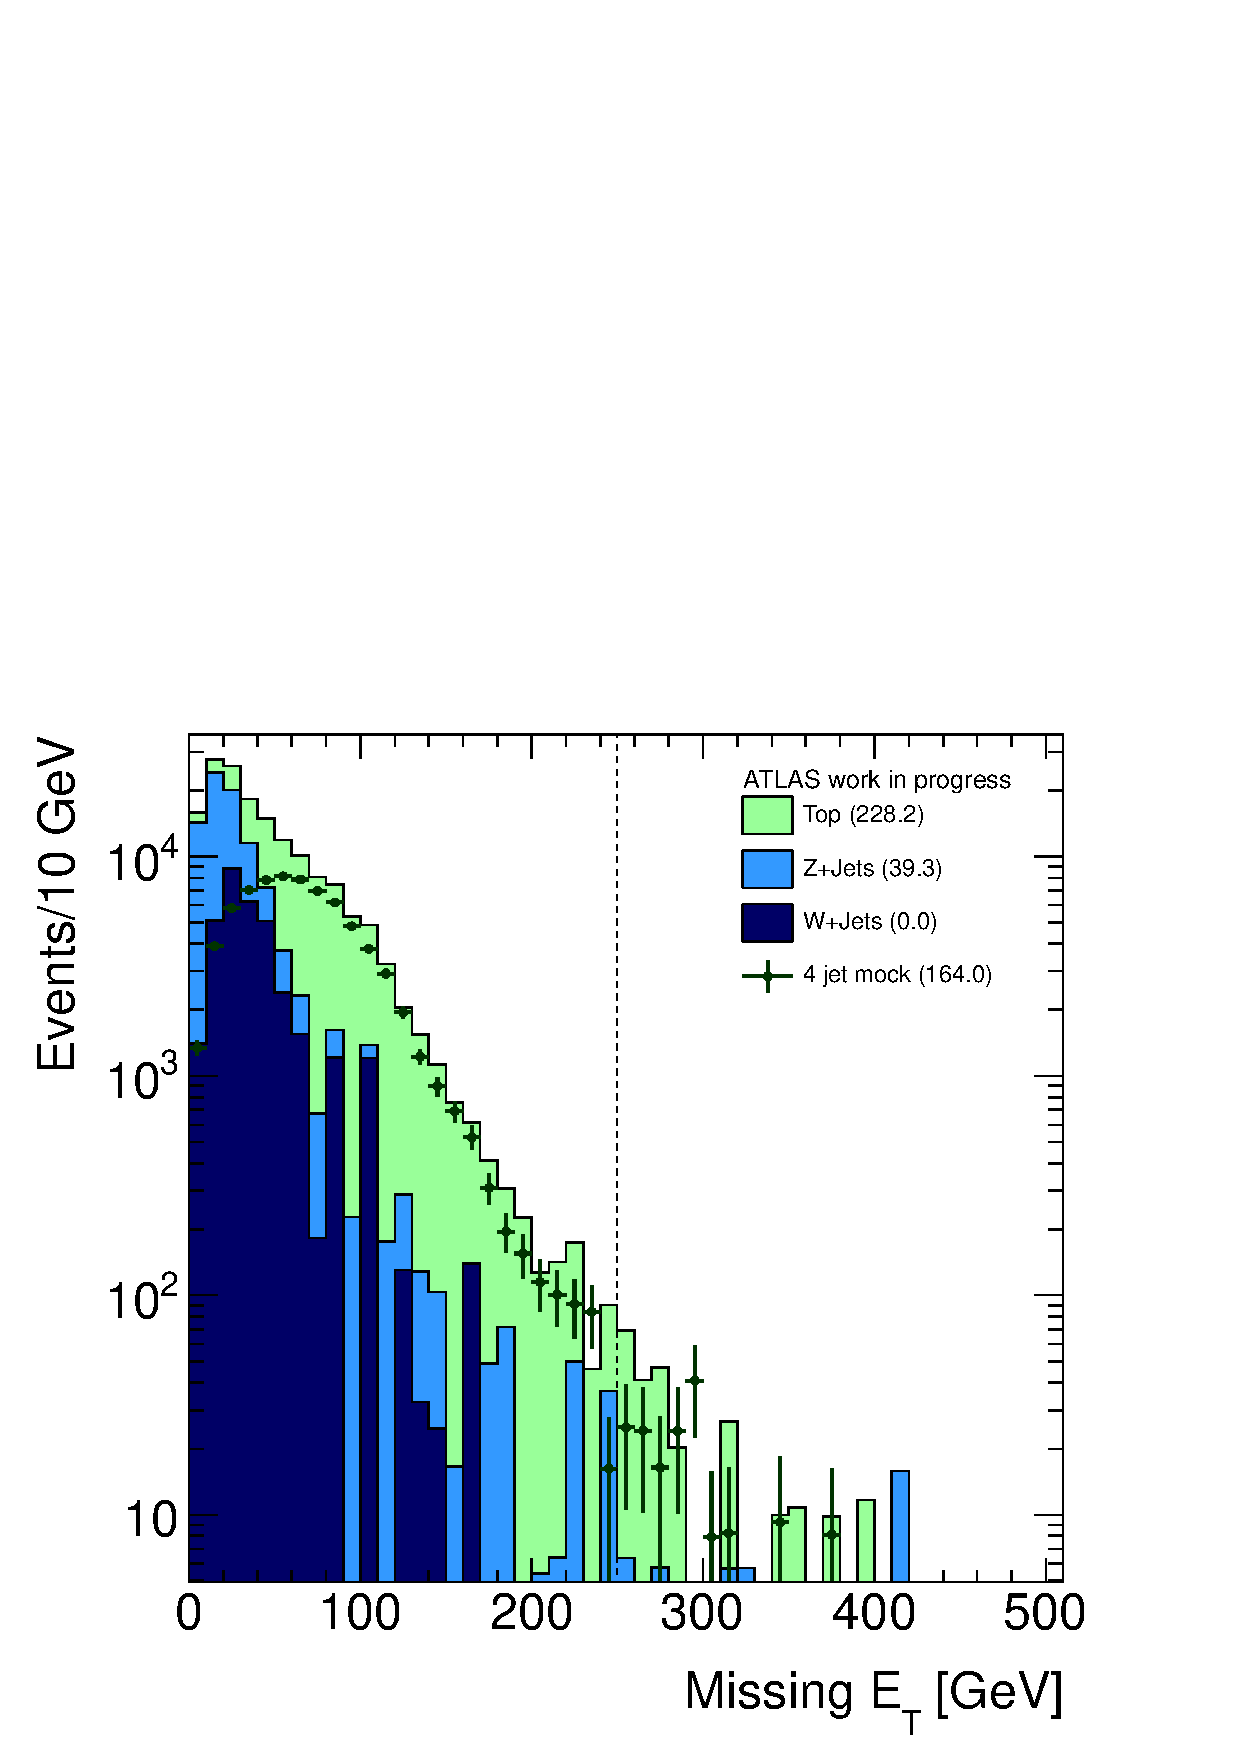
\includegraphics[scale=0.275]{img/Total_OS_EM_etmiss_scaled.pdf}
    \end{figure}\end{column}
    \begin{column}{0.45\textwidth}\begin{figure}
      \caption{$\mu^{\pm}e^{\mp}$$\slashed{E}_{T}$}
      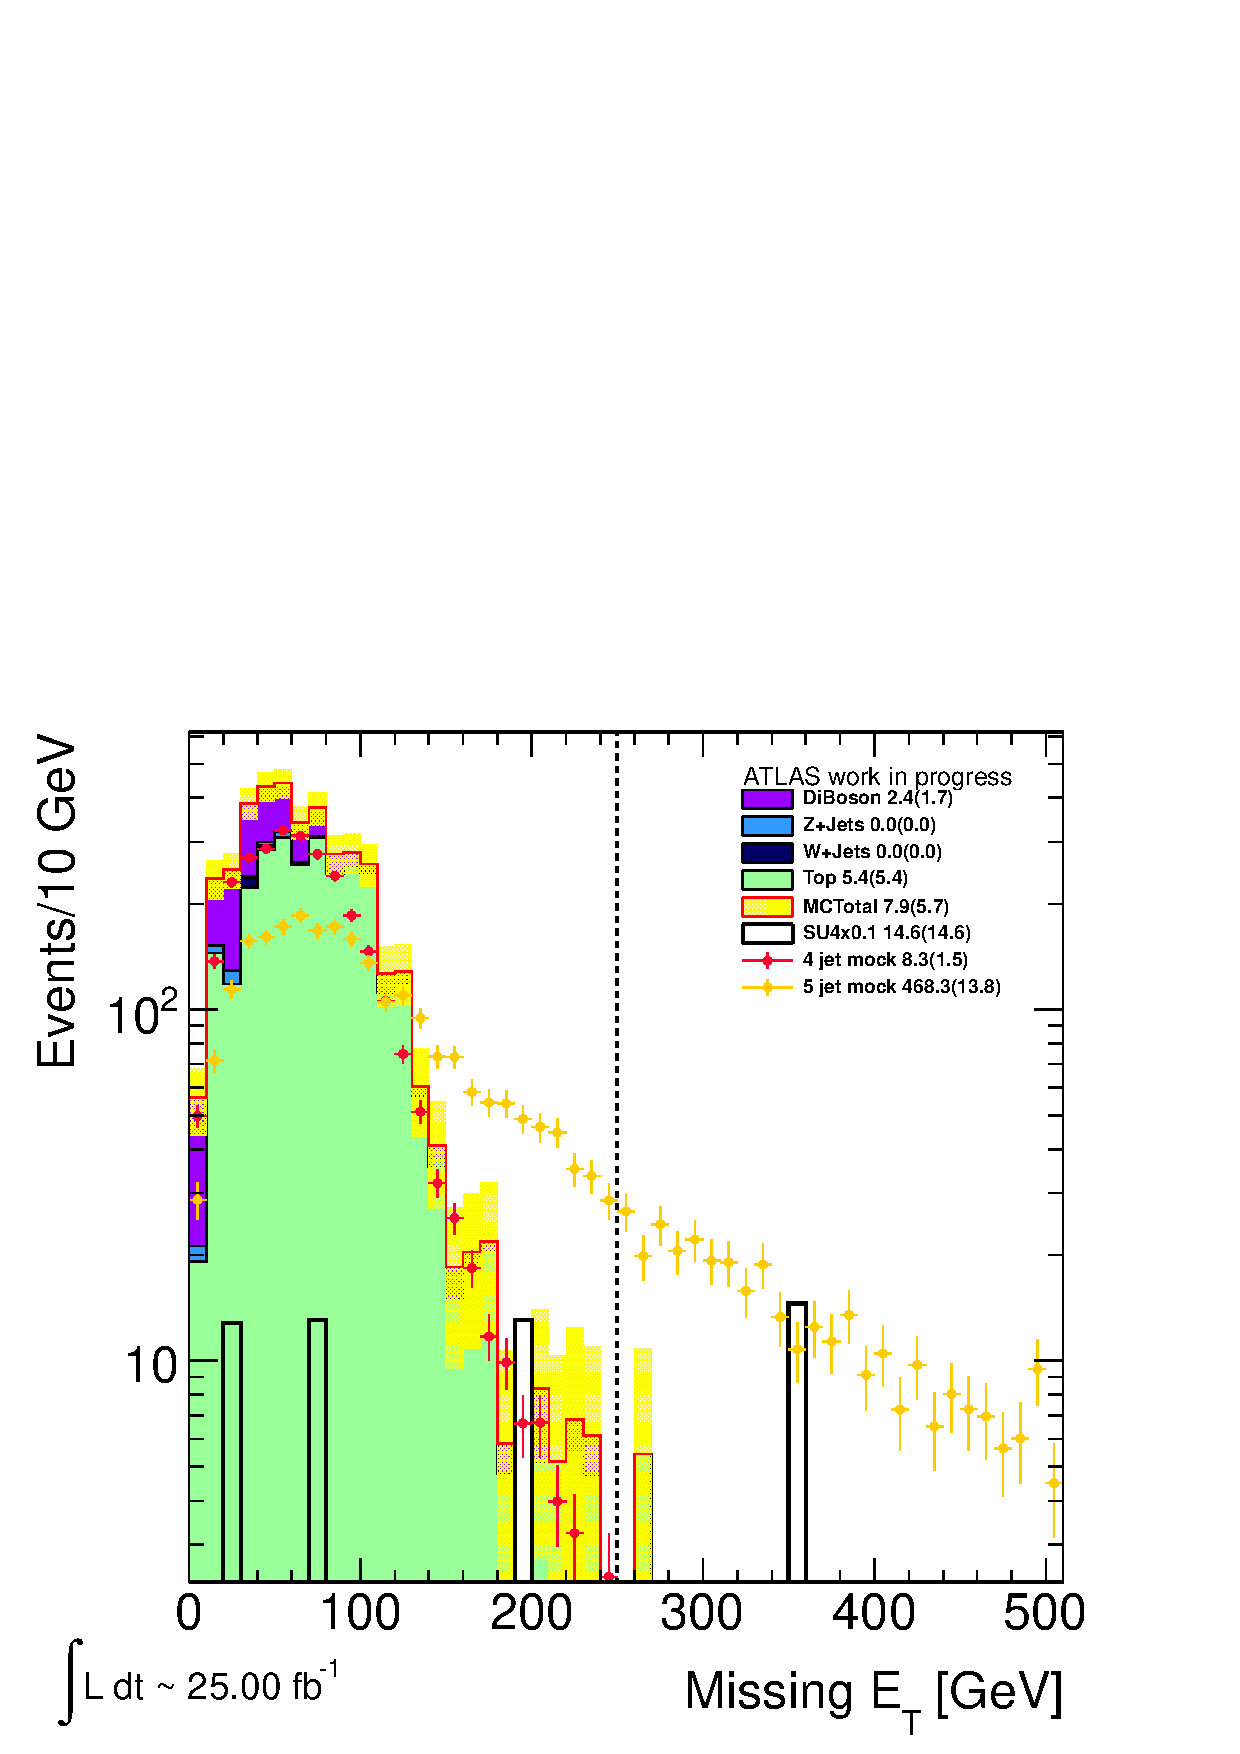
\includegraphics[scale=0.275]{img/Total_OS_ME_etmiss_scaled.pdf}
    \end{figure}\end{column}
  \end{columns}
\end{frame}

\begin{frame}{Jet pT - different flavour}
  \begin{columns}
    \begin{column}{0.45\textwidth}\begin{figure}
      \caption{$e^{\pm}\mu^{\mp}$$p_{T}^{\text{jet 1}}$}
      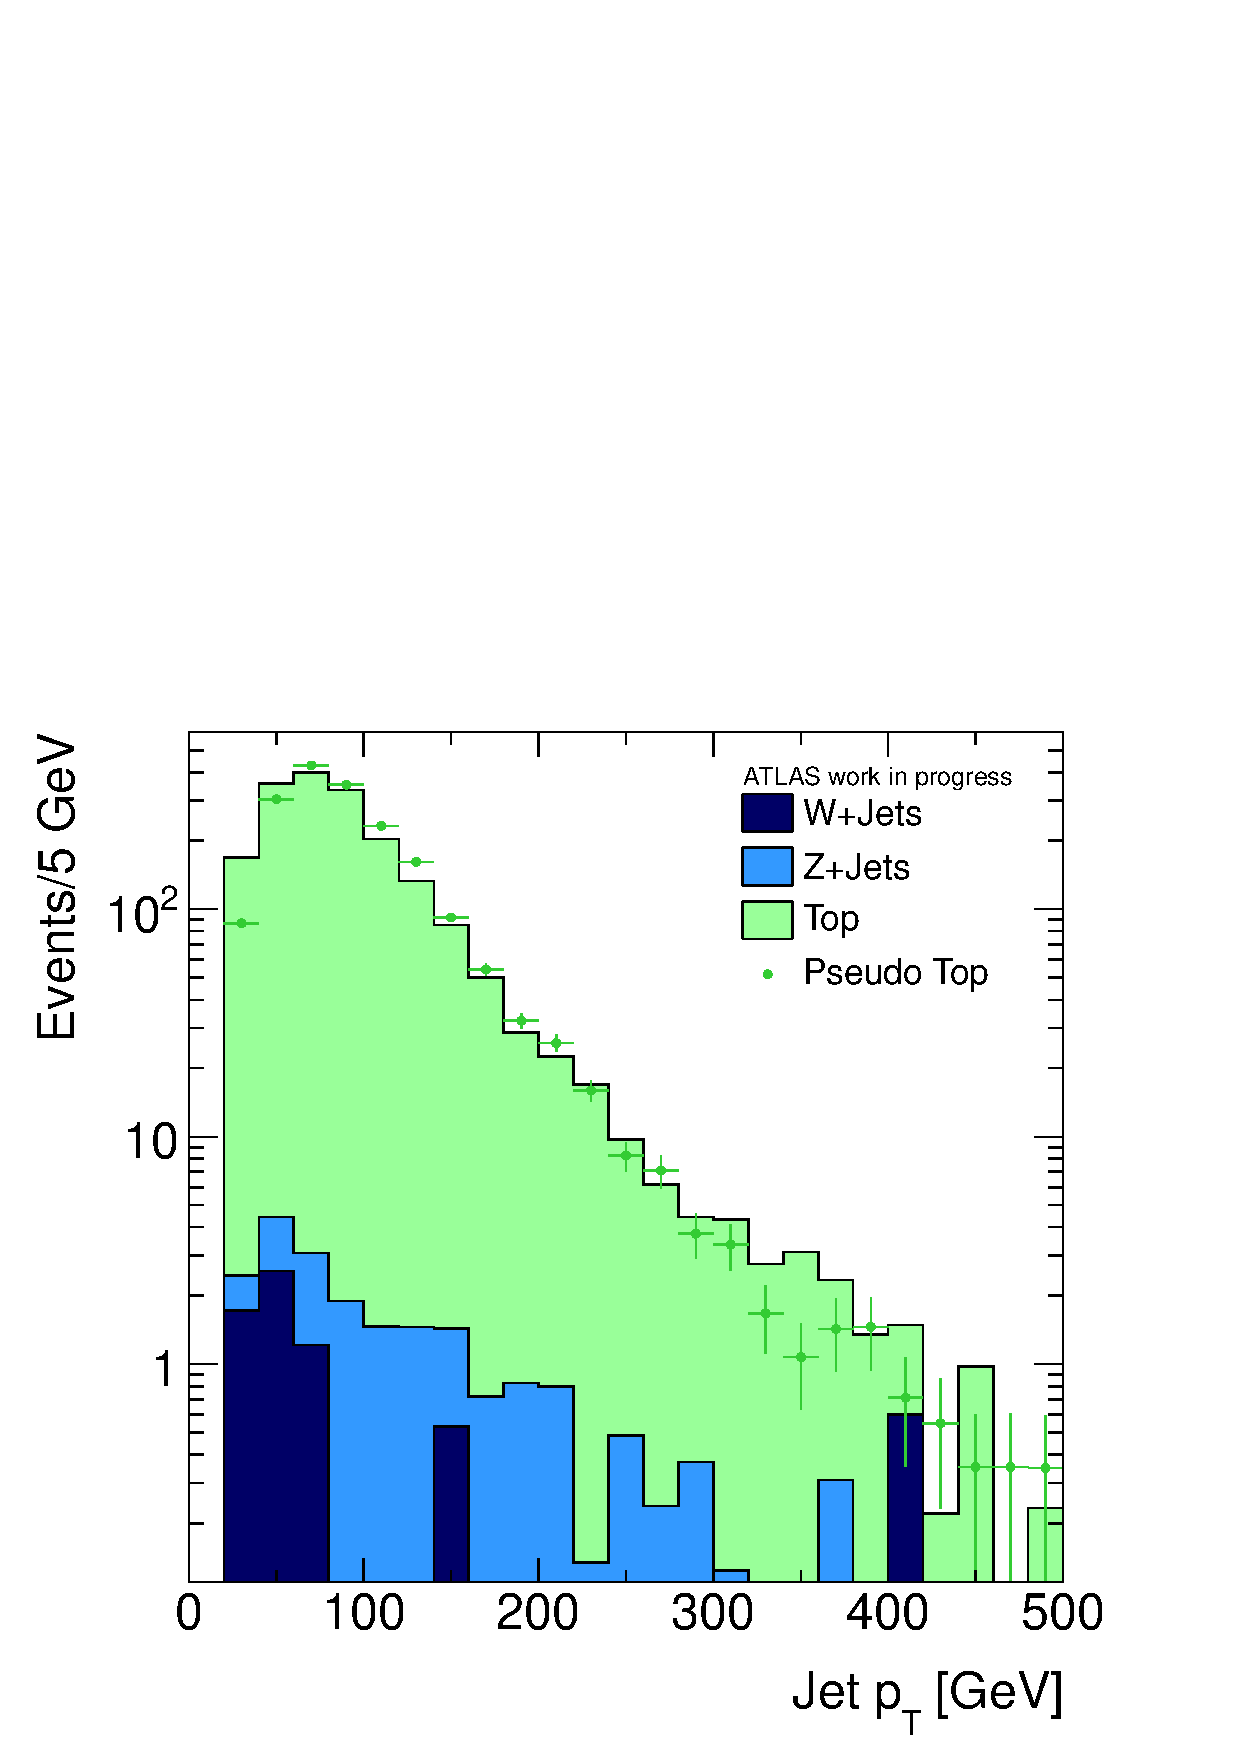
\includegraphics[scale=0.275]{img/Total_OS_EM_jet_lead_pt_scaled.pdf}
    \end{figure}\end{column}
    \begin{column}{0.45\textwidth}\begin{figure}
      \caption{$e^{\pm}\mu^{\mp}$$p_{T}^{\text{jet 2}}$}
      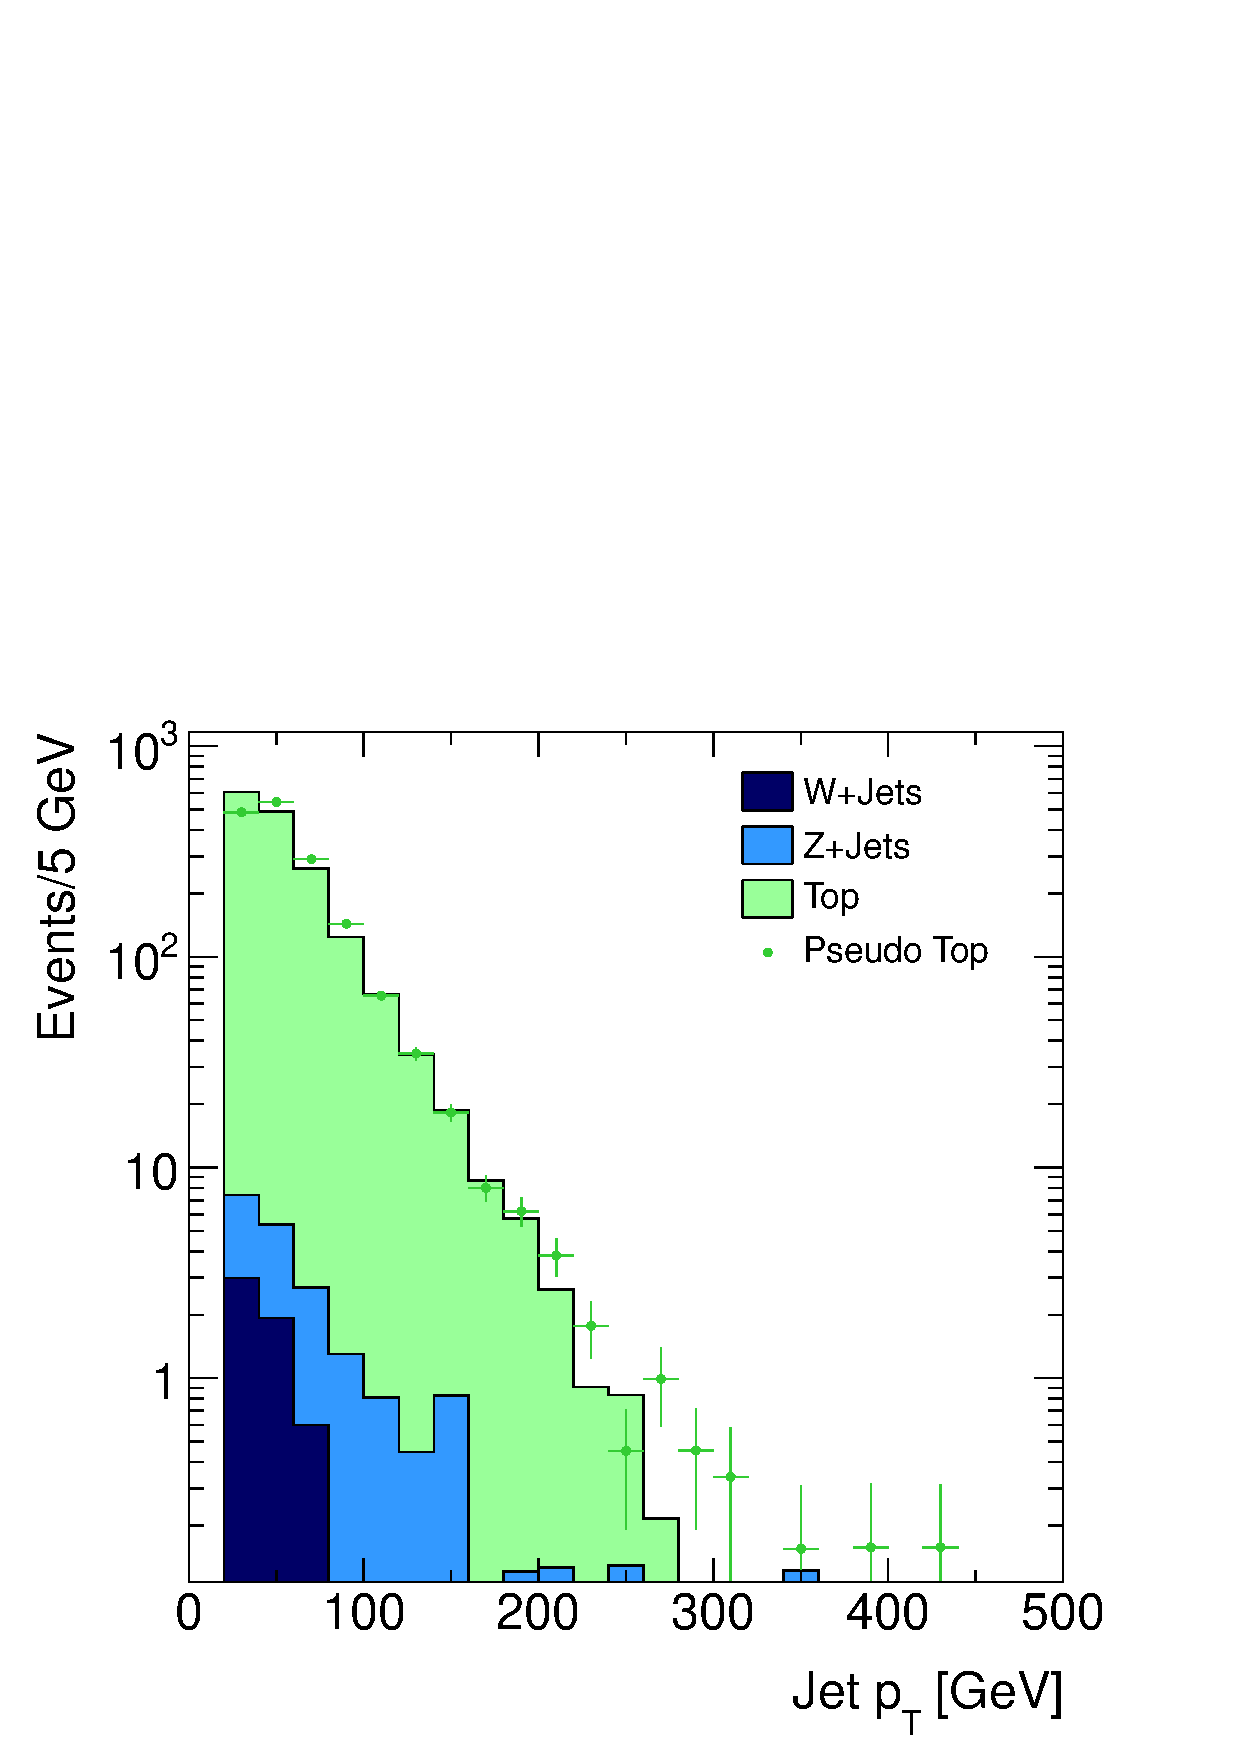
\includegraphics[scale=0.275]{img/Total_OS_EM_jet_lead2_pt_scaled.pdf}
    \end{figure}\end{column}
  \end{columns}
\end{frame}

\begin{frame}{Jet pT - different flavour}
  \begin{columns}
    \begin{column}{0.45\textwidth}\begin{figure}
      \caption{$\mu{\pm}e^{\mp}$$p_{T}^{\text{jet 1}}$}
      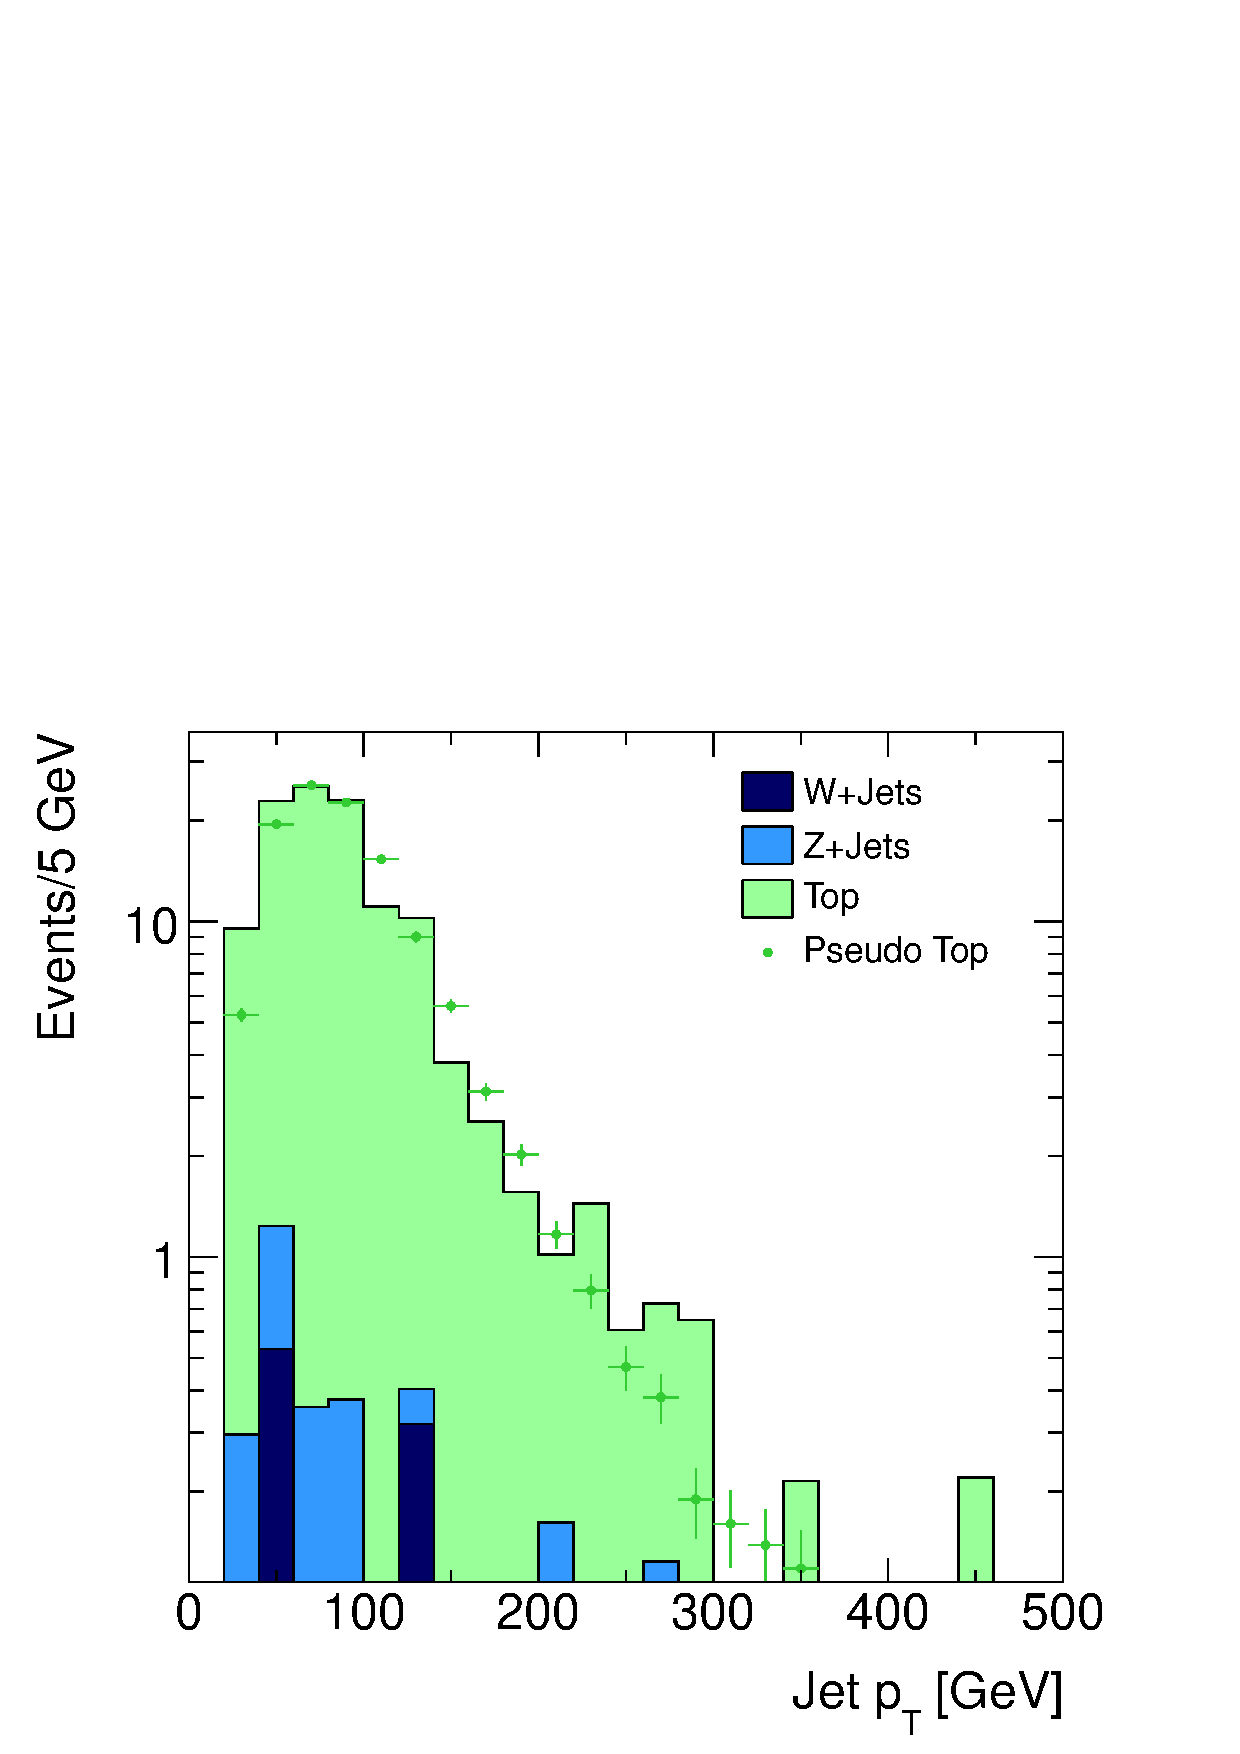
\includegraphics[scale=0.275]{img/Total_OS_ME_jet_lead_pt_scaled.pdf}
    \end{figure}\end{column}
    \begin{column}{0.45\textwidth}\begin{figure}
      \caption{$\mu{\pm}e^{\mp}$$p_{T}^{\text{jet 2}}$}
      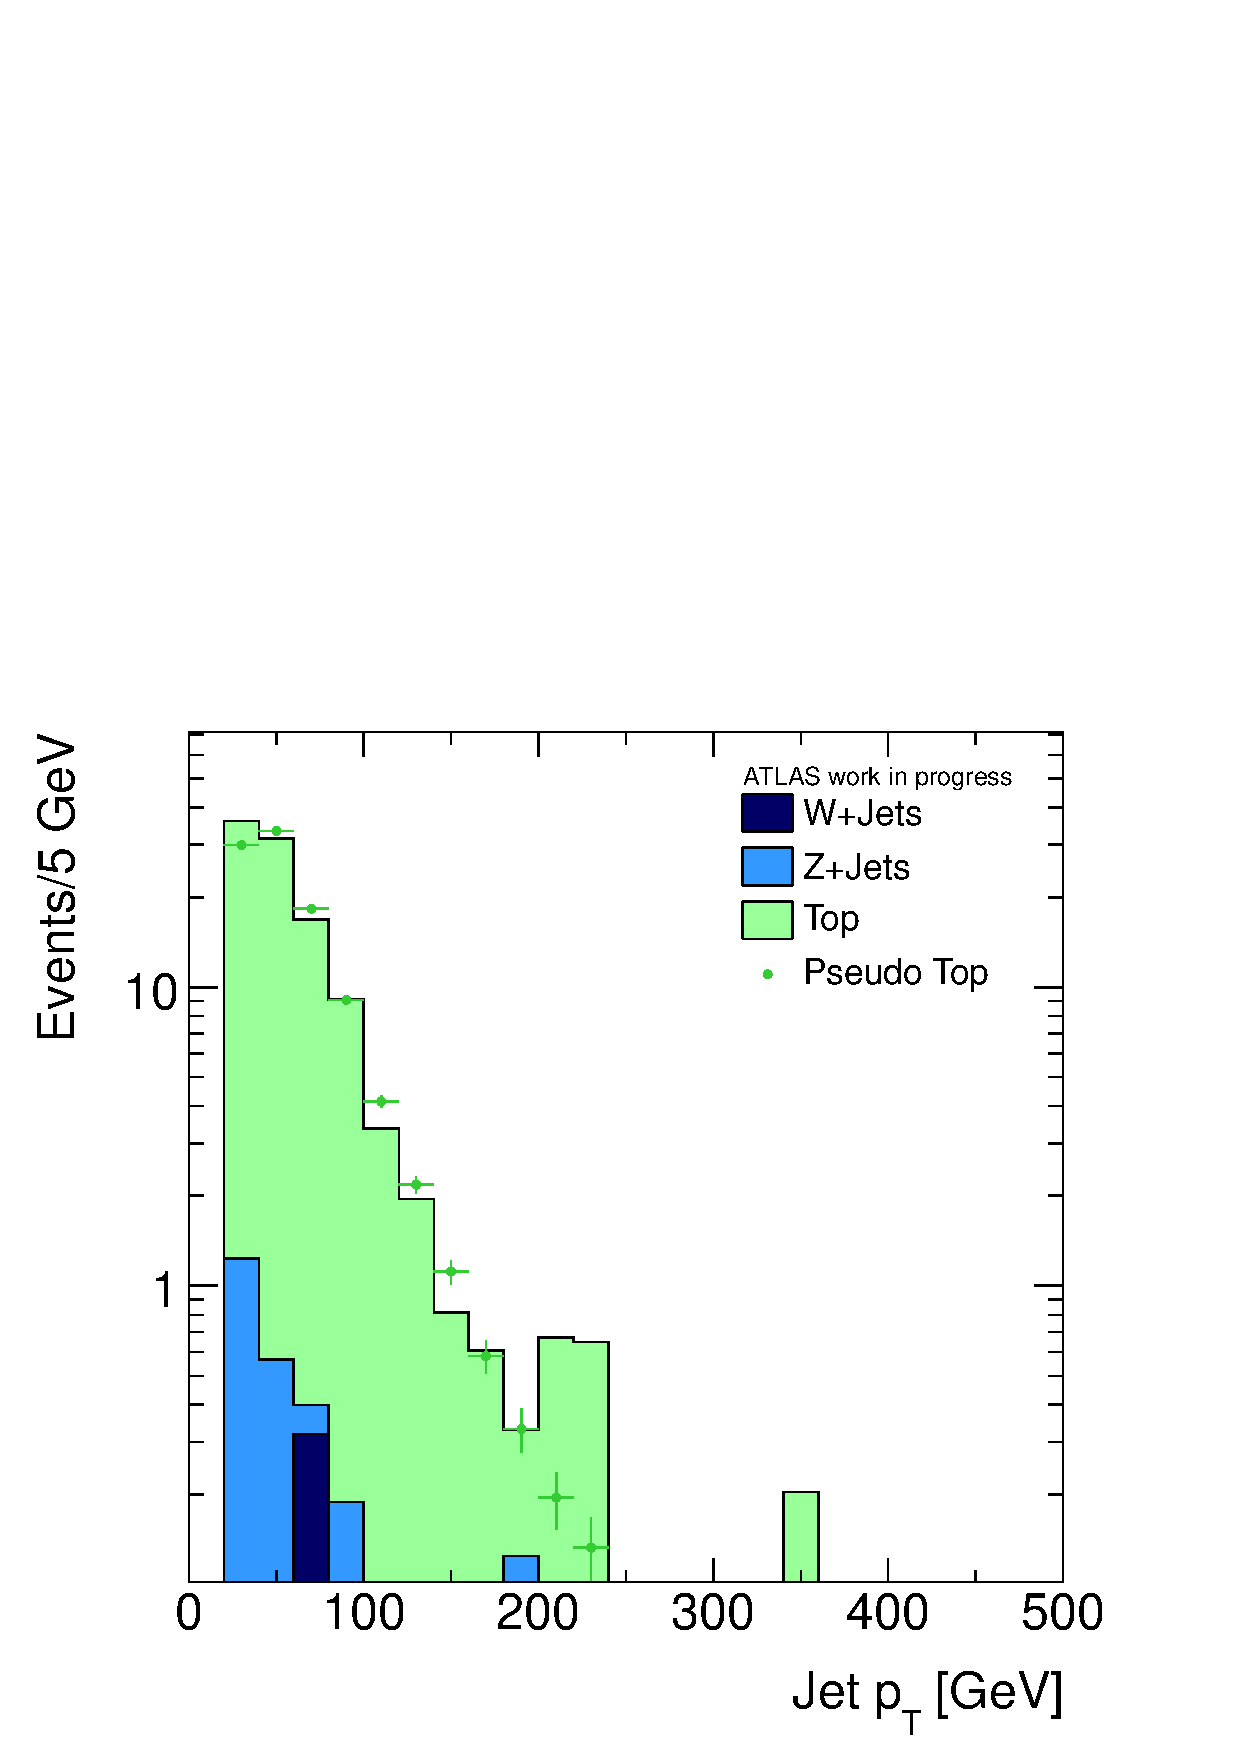
\includegraphics[scale=0.275]{img/Total_OS_ME_jet_lead2_pt_scaled.pdf}
    \end{figure}\end{column}
  \end{columns}
\end{frame}

\begin{frame}{Jet pT - muons}
  \begin{columns}
    \begin{column}{0.45\textwidth}\begin{figure}
      \caption{$\mu^{+}\mu^{-}$$p_{T}^{\text{jet 1}}$}
      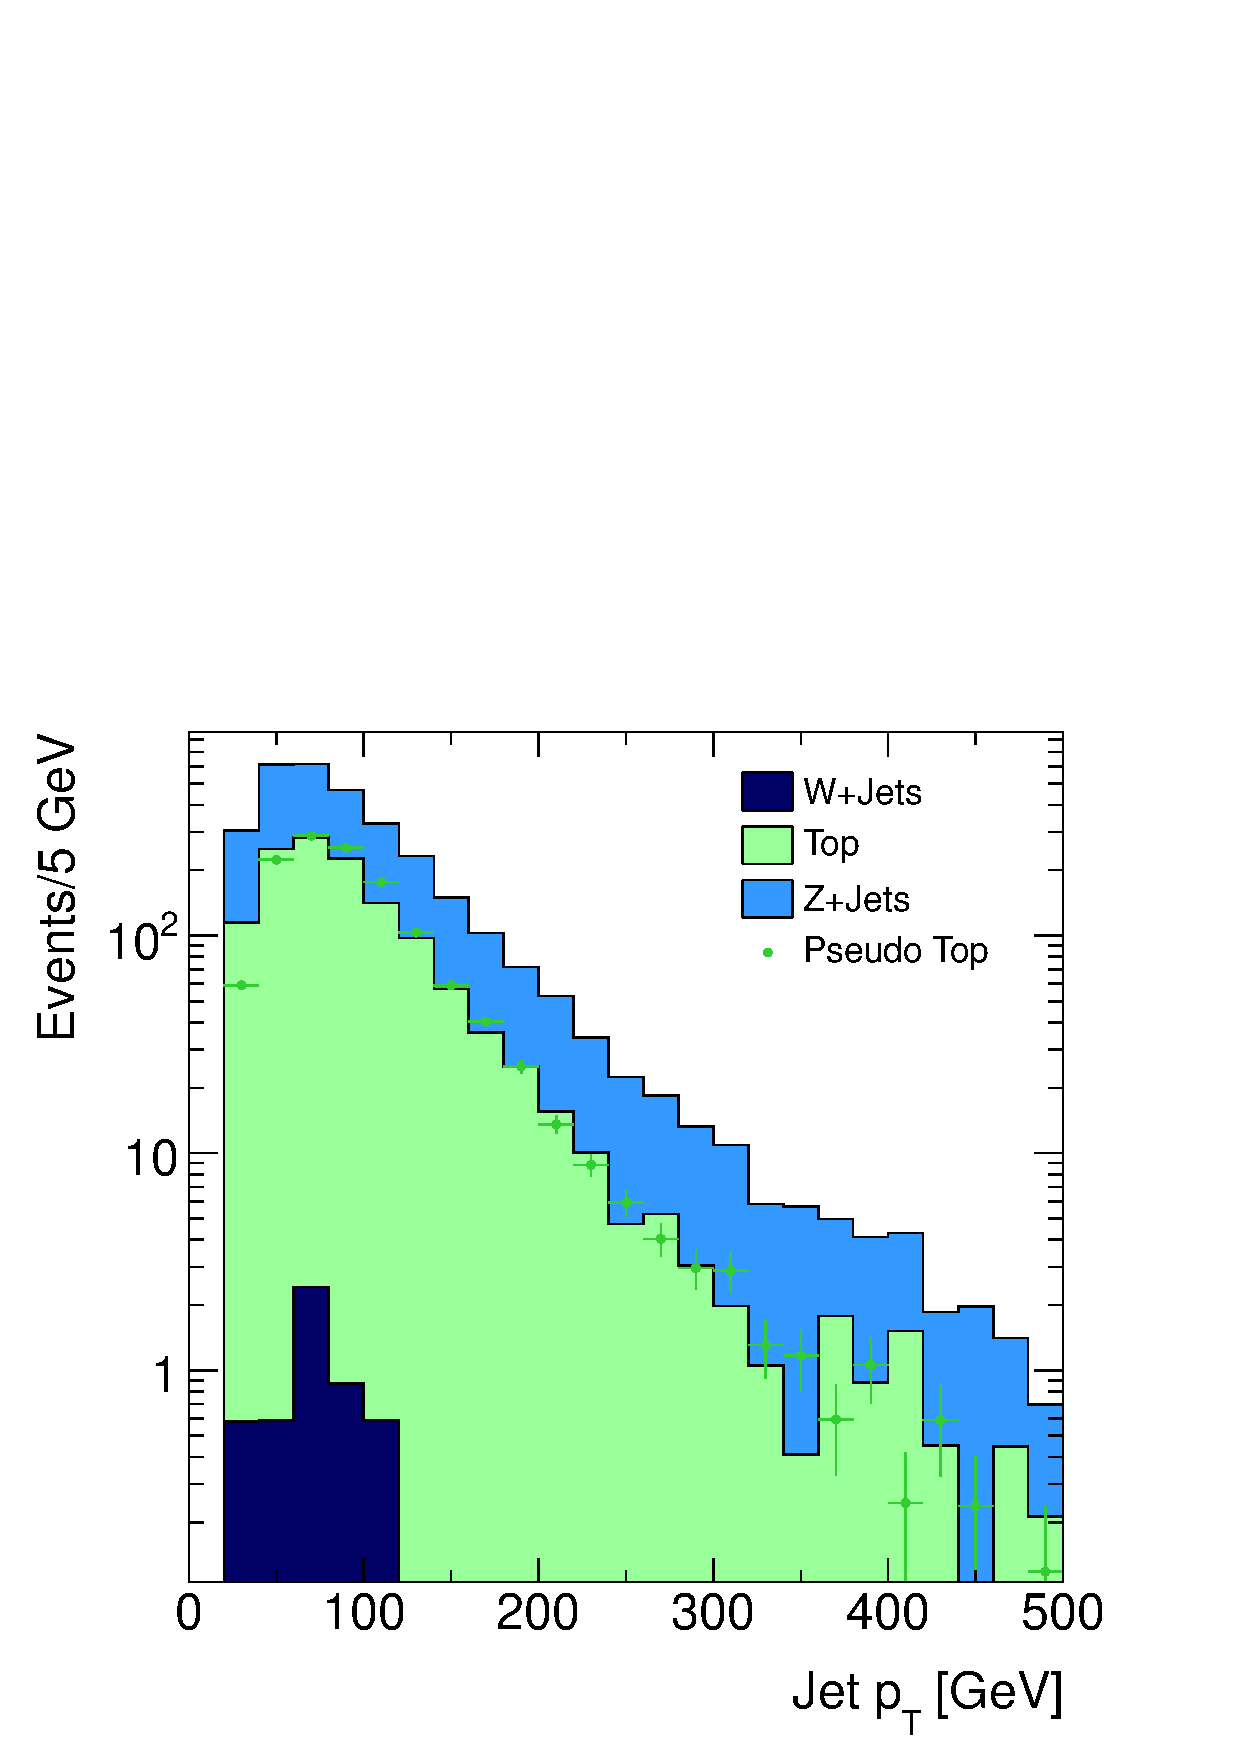
\includegraphics[scale=0.275]{img/Total_OS_MM_jet_lead_pt_scaled.pdf}
    \end{figure}\end{column}
    \begin{column}{0.45\textwidth}\begin{figure}
      \caption{$\mu^{+}\mu^{-}$$p_{T}^{\text{jet 2}}$}
      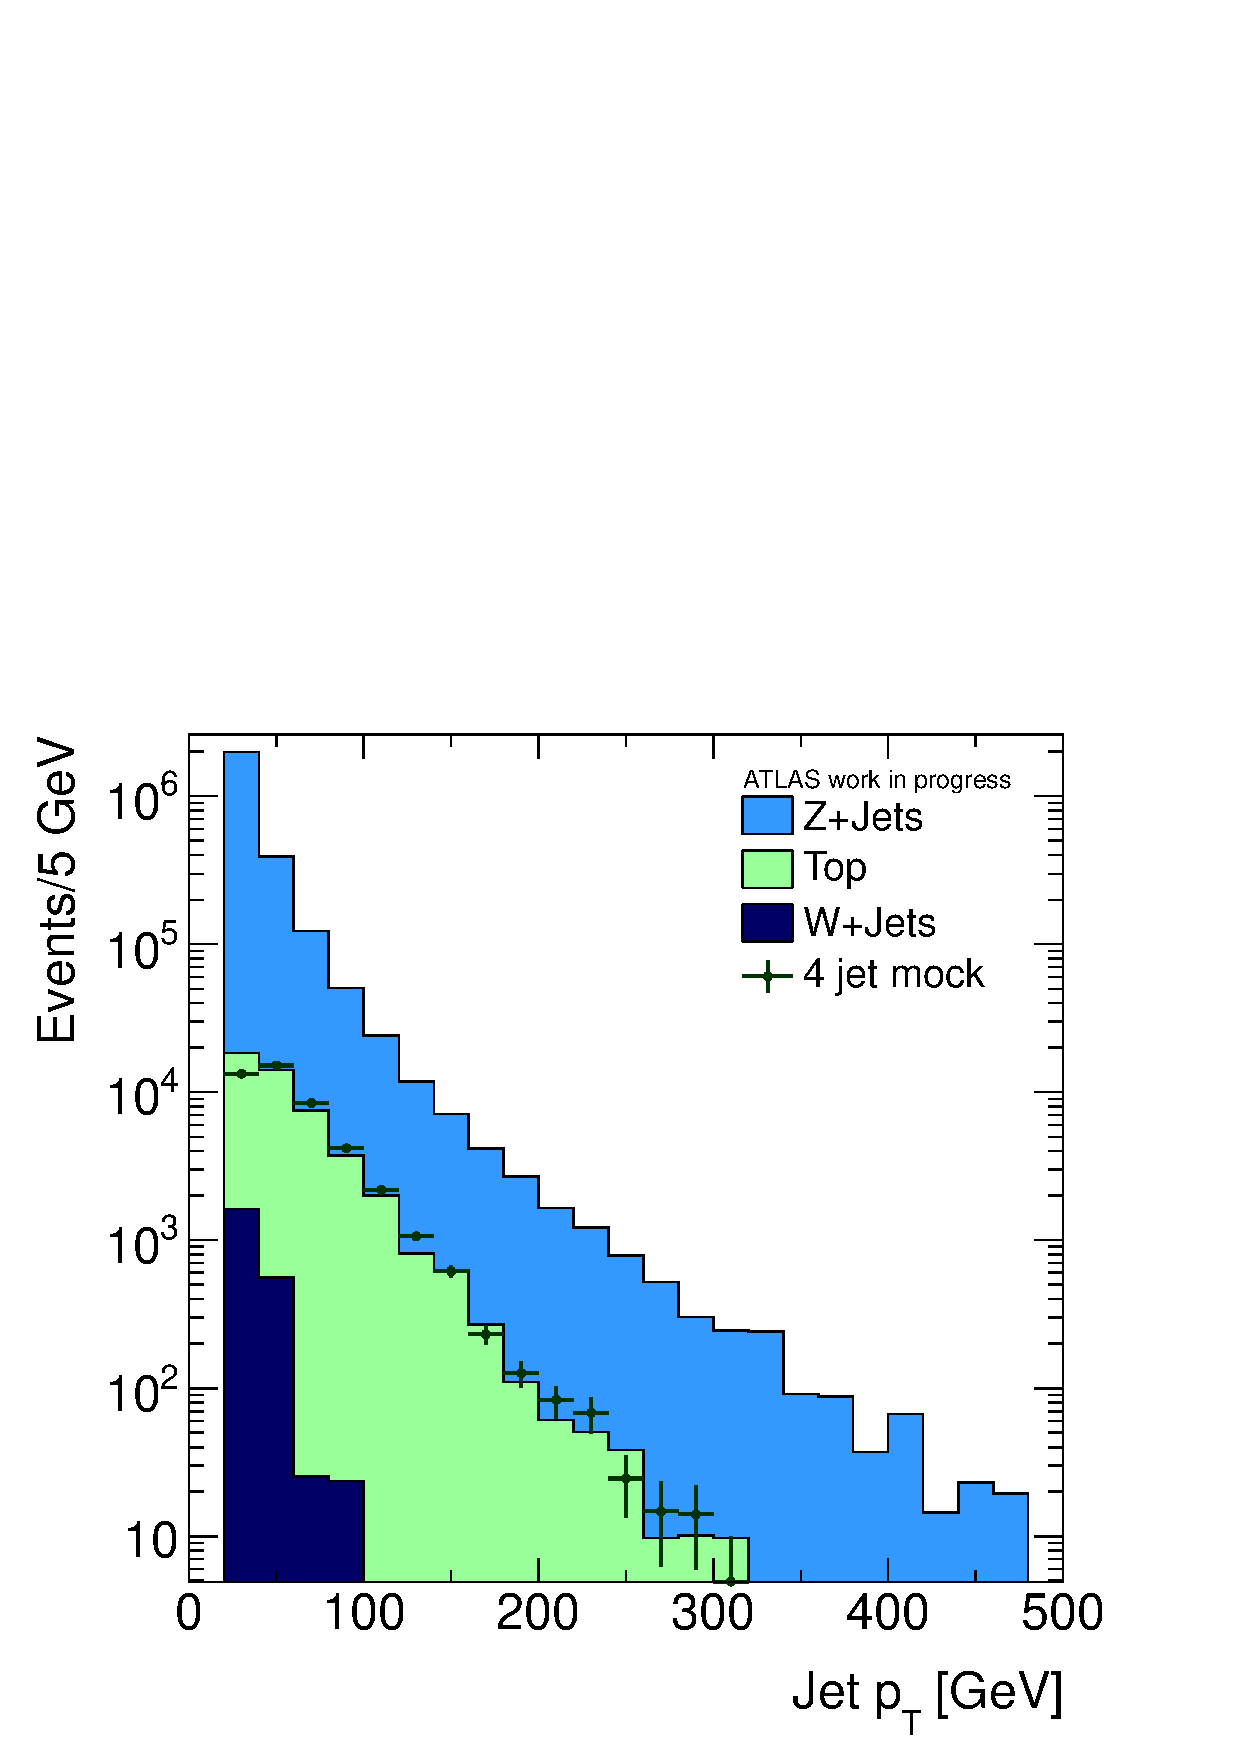
\includegraphics[scale=0.275]{img/Total_OS_MM_jet_lead2_pt_scaled.pdf}
    \end{figure}\end{column}
  \end{columns}
\end{frame}

\end{document}
